% interactnlmsample.tex
% v1.05 - August 2017

% \documentclass{interact}
\documentclass[largeformat]{interact}

\usepackage{epstopdf}% To incorporate .eps illustrations using PDFLaTeX, etc.
% \usepackage[caption=false]{subfig}% Support for small, `sub' figures and tables
% \usepackage[nolists,tablesfirst]{endfloat}% To `separate' figures and tables from text if required
%\usepackage[doublespacing]{setspace}% To produce a `double spaced' document if required
%\setlength\parindent{24pt}% To increase paragraph indentation when line spacing is doubled
\usepackage[numbers,sort&compress]{natbib}% Citation support using natbib.sty

%=================================================================
% ADDITIONAL PACKAGES
%=================================================================
\usepackage{url}            % Correct formatting of URLs (handles underscores, line breaks)
\usepackage{tabularx}       % Flexible-width tables with X column type
\usepackage{float}          % Precise float placement with [H] specifier
\usepackage{enumitem}       % Customizable enumerate/itemize spacing and labels
\usepackage{algorithm}      % Floating environment for algorithm blocks
\usepackage{algpseudocode}  % Structured pseudocode (algorithmicx-based)
\usepackage{orcidlink}      % Clickable ORCID identifiers for author names
\usepackage{subcaption}     % Subfigures and subtables within single float
\usepackage{listings}       % Source code typesetting with syntax highlighting
\usepackage{xcolor}         % Extended color support (for listings, tables, highlighting)
\usepackage{needspace}      % Prevent page breaks in inappropriate locations
\usepackage{multicol}       % Multiple column layout support
\usepackage{multirow}       % Table cells spanning multiple rows
\usepackage{longtable}      % Multi-page tables
\usepackage{booktabs}       % Professional table rules (\toprule, \midrule, \bottomrule)
\usepackage[table]{xcolor}  % Table cell background coloring (loads xcolor with table option)
\usepackage{array}          % Extended column type definitions
\usepackage{ragged2e}       % Better ragged text alignment (RaggedRight, Centering)
\usepackage{calc} % for width/height calculations
\usepackage{graphicx}
\usepackage{xurl}
\usepackage{graphicx}      % For \includegraphics
\usepackage{algorithm}     % For algorithm environment
% \usepackage{algorithmic}   % For algorithmic environment
\usepackage{xcolor}        % For colors
\usepackage{float}         % For [H] placement specifier
\usepackage{caption}
\captionsetup[figure]{font=footnotesize}
\captionsetup[algorithm]{font=small}

% Add to preamble:
\newcolumntype{T}{>{\ttfamily}l}  % Monospace left-aligned
\newcolumntype{M}[1]{>{\ttfamily}p{#1}}  % Monospace paragraph
%=================================================================
% LONGTABLE CONFIGURATION
%=================================================================
\setlength{\LTleft}{0pt}    % Remove left indentation for longtables
\setlength{\LTright}{0pt}   % Remove right indentation for longtables

%=================================================================
% COLOR DEFINITIONS
%=================================================================
% General table styling
\definecolor{rowgray}{gray}{0.96}   % Subtle row striping for alternating rows

% Error class colors (light, print-safe)
\definecolor{ecorrect}{RGB}{226,245,233}  % Light green - correct answers
\definecolor{epartial}{RGB}{255,243,205}  % Light yellow - partial answers
\definecolor{ehalluc}{RGB}{248,215,218}   % Light red/pink - hallucinations
\definecolor{efield}{RGB}{207,226,255}    % Light blue - field errors
\definecolor{eparser}{RGB}{233,236,239}   % Light gray - parser errors

% RCP column highlight
\definecolor{ercp}{RGB}{238,242,255}      % Very light indigo/blue for RCP column

%=================================================================
% CUSTOM MACROS
%=================================================================
% RCP cell background tint
\newcommand{\rcpcell}[1]{\cellcolor{ercp}{#1}}

% Error class badge: \errcell{<color>}{<text>}
\newcommand{\errcell}[2]{\cellcolor{#1}#2}

%=================================================================
% CUSTOM COLUMN TYPES
%=================================================================
\newcolumntype{L}[1]{>{\RaggedRight\arraybackslash}p{#1}}  % Left-aligned ragged column
\newcolumntype{C}[1]{>{\Centering\arraybackslash}p{#1}}    % Centered column

%=================================================================
% BIBLIOGRAPHY CONFIGURATION (natbib)
%=================================================================
\bibpunct[, ]{[}{]}{,}{n}{,}{,}     % Citation format: [1, 2, 3]
\renewcommand\bibfont{\fontsize{10}{12}\selectfont}  % Bibliography font size: 10pt/12pt leading

\makeatletter
\def\NAT@def@citea{\def\@citea{\NAT@separator}}  % Suppress spaces between citations
\makeatother

%=================================================================
% THEOREM ENVIRONMENTS (amsthm)
%=================================================================
\theoremstyle{plain}                % Theorem style (italic body text)
\newtheorem{theorem}{Theorem}[section]
\newtheorem{lemma}[theorem]{Lemma}
\newtheorem{corollary}[theorem]{Corollary}
\newtheorem{proposition}[theorem]{Proposition}

\theoremstyle{definition}           % Definition style (upright body text)
\newtheorem{definition}[theorem]{Definition}
\newtheorem{example}[theorem]{Example}

\theoremstyle{remark}               % Remark style (upright body text)
\newtheorem{remark}{Remark}
\newtheorem{notation}{Notation}
%=================================================================

\begin{document}
\articletype{Research Article} % Specify the article type or omit as appropriate
\title{A Domain-Agnostic Agentic Architecture for Structured Extraction of Engineering Knowledge}
\author{
    \name{
    Oscar Ikechukwu\textsuperscript{a}\thanks{CONTACT Oscar Ikechukwu. Email: oscar.ikechukwu@liu.se},
    Mehdi Tarkian\textsuperscript{a},
    Sanjay Nambiar\textsuperscript{a},
    Marie Jonsson\textsuperscript{a},
    Christoffer Brax\textsuperscript{b}
    }
    \affil{\textsuperscript{a}
    % Division of Product Realization, Department of Management and Engineering,
    % Link\"oping University, Link\"oping, Sweden,\\
    Division of Product Realization, IEI,
    Link\"oping University, Link\"oping, Sweden\\
    \textsuperscript{b}
    Saab Surveillance, Saab AB, Link\"oping, Sweden
    }
}
%=================================================================
% \tableofcontents
% \listoftables
% \listoffigures
%=================================================================
\maketitle
%=================================================================
\begin{abstract}
Engineering organizations increasingly adopt large language models (LLMs) to retrieve facts from heterogeneous technical documentation; however, deployments remain brittle when answers must be grounded to specific sections, pages, and tabular data in documentation. In practice, retrieval-augmented generation and agent pipelines often fail due to hallucinations, weak validation, and limited traceability, especially in table-dense and revision-controlled engineering corpora. This paper presents an applied, domain-agnostic agentic architecture for structured extraction and verification of engineering knowledge. The approach introduces a persistent, SQL-backed Relational Control Plane (RCP) that stores goals, strategies, tool calls, outputs, and validation outcomes as first-class relational entities. The design goal is to integrate and support governance by storing every intermediate artifact and check result. Reasoning is organized as a six-stage loop (goal definition, strategy selection, agent execution, agent validation, strategy validation, and goal validation) that enforces evidence-centric progression and enables deterministic replay and audit-ready provenance. We evaluate the framework on two industrial case studies involving a hydraulic product catalogue and revision-controlled technical documentation. Compared to baseline retrieval and non-validated agent pipelines, the proposed architecture improves citation and revision fidelity, reduces unsupported generations, and provides transparent, queryable execution traces. These results demonstrate a practical pathway for deploying trustworthy generative-AI systems in engineering knowledge management.
\end{abstract}

%=================================================================
\begin{keywords}
Agentic AI; Engineering Informatics; Large Language Models; Knowledge Engineering
\end{keywords}

%=================================================================
% \begin{abbreviations}
% AI -- Artificial intelligence\\
% CAD -- Computer-aided design\\
% LLM -- Large language model\\
% OCR -- Optical character recognition\\
% PLM -- Product lifecycle management\\
% RAG -- Retrieval-augmented generation\\
% RCP -- Relational control plane\\
% SQL -- Structured query language
% \end{abbreviations}


%%%%%%%%%%%%%%%%%%%%%%%%%%%%%%%%%%%%%%%%%%%%%%%%%%%%%%%%%%%%%%%%%%%%%%%%%%%%%%%%%%%%%%%%%%%%%%%%%%%%%%
% INTRODUCTION
%%%%%%%%%%%%%%%%%%%%%%%%%%%%%%%%%%%%%%%%%%%%%%%%%%%%%%%%%%%%%%%%%%%%%%%%%%%%%%%%%%%%%%%%%%%%%%%%%%%%%%
\section{Introduction}
\label{sec:Introduction}
% \textcolor{red}{Introduction}

Recent advances in large language models (LLMs) have intensified efforts to operationalize institutional knowledge across complex enterprise data ecosystems \cite{yamsani2025stewardship}. Engineering organizations routinely retrieve precise product, component, and process details by cross-referencing heterogeneous documentation—specifications, drawings, standards, service manuals, part-revision histories, and engineering change orders (ECO/ECN)—tasks that traditionally require years of domain expertise. Industrial studies have begun to illustrate the potential of LLM-based tools to support engineering knowledge sharing. For example, Freire et al.~\cite{kernanfreire2024knowledge} developed an LLM-driven Q\&A system that integrates factory documentation with expert operator knowledge. The system answers operator queries by searching relevant manuals and reports, significantly accelerating information retrieval in manufacturing settings, while also underscoring the continued need for expert validation.

Retrieval-Augmented Generation (RAG) improves access to such domain knowledge \cite{lewis2020rag}; however, current pipelines remain brittle in engineering contexts. They frequently hallucinate, struggle with multi-document reasoning, and underperform on non-text modalities common in technical documentation—including dense tables, figures, engineering drawings, CAD callouts, and scanned PDFs \cite{huang2025hallucinationsurvey, kalai2025hallucinate}. Advanced RAG approaches such as RAPTOR construct hierarchical representations of long documents and retrieve information at multiple abstraction levels, improving cross-chunk coherence and reducing irrelevant context \cite{sarthi2024raptor}. Nevertheless, several challenges persist in engineering applications: (i) revision and change awareness, where answers must reflect the correct revision scope and supersession rules; (ii) table and units fidelity, since critical information often resides in dense tables requiring robust parsing and normalization; (iii) cross-constraint reasoning across bills of materials (BOMs), ECOs, service bulletins, and standards; and (iv) provenance traceability to exact clauses, figures, or table cells for auditability \cite{pan2025multimodalKG}.

Agentic frameworks mitigate some of these limitations by orchestrating tools, multi-step planning, and verification (e.g., ReAct-style reasoning-and-acting \cite{yao2023reactsynergizingreasoningacting}; tool-use learning \cite{schick2023toolformerlanguagemodelsteach}).  In engineering contexts, however, no single agent typically suffices. Depending on domain and task, systems must coordinate specialized components—such as a table/units agent for numerical extraction and normalization, a revision/lineage agent for change tracking, a CAD/PLM agent for configuration reasoning, and a standards agent for normative rule interpretation. This coordination significantly increases the burden of managing system state, execution flows, retries, and observability. Frameworks such as LangGraph provide useful abstractions, but production deployments still require explicit state design, graph orchestration, heterogeneous tool integration (e.g., vector stores, OCR systems, table parsers, CAD/PLM APIs), persistence, evaluation, and replay \cite{langgraph_docs}.

This paper presents a domain-agnostic agentic framework for orchestrating multi-agent reasoning workflows across engineering knowledge domains. The central novelty lies in externalizing orchestration state into a relational persistence model backed by SQL. Rather than maintaining transient in-memory execution graphs, all orchestration artifacts—goals, strategies, agent calls, parameters, outputs, and validation outcomes—are stored as structured relational records, enabling deterministic replay, full observability, and audit-ready traceability. By decoupling orchestration policies from retrieval implementations and remaining partially independent of specific vector-store technologies, the framework achieves modularity, adaptability, and operational simplicity.

Empirical evaluations on engineering document retrieval and reasoning tasks demonstrate that the proposed architecture preserves the benefits of multi-step retrieval and tool use while reducing hallucination rates through structured validation. Beyond accuracy improvements, the system produces audit-ready execution traces that support governance and reproducibility in industrial settings where incorrect units, revision scope, or missing provenance can lead to costly downstream errors.

\noindent The contributions of this work are threefold:
\begin{itemize}[label=-]
    \item A validation-centric agentic architecture backed by a persistent Relational Control Plane (RCP), in which goals, strategies, function invocations, and validation outcomes are stored as queryable relational records—enabling deterministic replay and governance-ready auditability.
    \item A domain-agnostic instantiation methodology, comprising reusable Strategy and Function Libraries, demonstrated across two fundamentally different industrial domains (catalogue-based product reasoning and revision-controlled document retrieval) without modification to the core orchestration logic.
    \item An empirical evaluation on 50 engineering queries comparing the RCP framework against RAG and non-persistent agentic baselines, demonstrating improved answer correctness and reduced hallucination with transparent, queryable execution traces.
\end{itemize}

% OLD SECTION 2
%%%%%%%%%%%%%%%%%%%%%%%%%%%%%%%%%%%%%%%%%%%%%%%%%%%%%%%%%%%%%%%%%%%%%%%%%%%%%%%%%%%%%%%%%%%%%%%%%%%%%%
% \section{State of the Art \textcolor{red}{(Under Construction)}}
% \label{sec:State of the Art}
%%%%%%%%%%%%%%%%%%%%%%%%%%%%%%%%%%%%%%%%%%%%%%%%%%%%%%%%%%%%%%%%%%%%%%%%%%%%%%%%%%%%%%%%%%%%%%%%%%%%%%
% \subsection{Agentic AI in Manufacturing}
% \label{subsec:Agentic AI in Manufacturing}

% Agentic AI systems are characterized by autonomous decision‑making, goal‑oriented action, and coordination among multiple agents, often operating with limited supervision in dynamic environments \cite{lim2024large,jafari2025measurement}. Unlike traditional AI rule‑based or single‑model classification—agentic AI uses reinforcement learning, multi‑agent systems (MAS), and LLMs to continuously reason, plan, and act in response to changing conditions \cite{olujimi2025agentic}.

% LLMs are used to extract design knowledge from engineering documents. Nicholson et al. (2025) evaluate GPT-4V (a vision-enabled LLM) on extracting information from 2D mechanical drawings. In one experiment, GPT-4V could describe a part and correctly read off five key dimensions from a drawing \cite{picard2025concept}. It then generated CAD scripts (in CadQuery, FeatureScript, OpenSCAD) to model the part, iteratively refining errors. This shows that VLMs can partially automate drawing interpretation and CAD generation, though the authors note that GPT-4V’s limited short-term memory required corrective feedback in multiple prompts \cite{picard2025concept}. In document knowledge management, Freire et al. (2024) build an LLM-based Q\&A system that ingests a factory’s documentation and operator knowledge. Their system answers operator queries by searching manuals and past logs. A user study found that the LLM tool dramatically sped up information retrieval and problem resolution, though workers still preferred human mentors when available \cite{freire2024knowledge}. These results emphasize the promise of LLMs for mining engineering knowledge, as well as the ongoing need for careful validation of the answers they provide.

% Another challenge is hallucination and factual grounding. VLMs like GPT-4V and GPT-4 are prone to “hallucinating” plausible-sounding but incorrect details \cite{gkournelos2024llm}. Systems try to mitigate this by using external knowledge sources: for example, Gkournelos et al. embed the LLM in a digital twin and knowledge base. They explicitly give the agent access to “manufacturing proprietary knowledge bases” and live data via a digital twin, so it can verify its outputs \cite{gkournelos2024llm}. A related issue is the limited context and memory of LLM agents. Most systems use one or two conversational agents with fixed context windows. Nicholson et al. found that even GPT-4V loses track of earlier details when prompted iteratively through many CAD corrections \cite{picard2025concept}. Singh et al. note that continuous processes (batch vs continuous) may require “more reprompts” and that LLMs’ finite context will limit how much of the system model can be processed at once \cite{singh2025leveraging}. They suggest RAG as a solution to feed the LLM only the necessary structured slices of the digital twin \cite{singh2025leveraging}. In practice, this means splitting knowledge into a database or memory store and having LLM agents fetch relevant facts as needed.

% There is a challenge in integrating agentic AI with formal validation frameworks or redundant checks to catch erroneous agent outputs before they cause defects. The literature shows a rapid rise of multi-agent, LLM-driven automation for engineering. These systems demonstrate the potential of agentic AI to improve flexibility and autonomy. Yet they also reveal gaps: existing methods often scale only to narrow tasks, rely on fixed architectures, and incur hallucinations without grounding. Future research must tackle these gaps by designing truly dynamic agent systems, embedding structured knowledge (databases, digital twins) for LLMs, and building rigorous validation layers. As multiple researchers observe, combining LLM reasoning with dedicated knowledge resources and modular agent coordination is essential for safe, scalable manufacturing automation.


%%%%%%%%%%%%%%%%%%%%%%%%%%%%%%%%%%%%%%%%%%%%%%%%%%%%%%%%%%%%%%%%%%%%%%%%%%%%%%%%%%%%%%%%%%%%%%%%%%%%%%
% RELATED WORK
%%%%%%%%%%%%%%%%%%%%%%%%%%%%%%%%%%%%%%%%%%%%%%%%%%%%%%%%%%%%%%%%%%%%%%%%%%%%%%%%%%%%%%%%%%%%%%%%%%%%%%
\section{Related work}
\label{sec:related_work}

%==============================================================================
\subsection{Agentic AI in Engineering}
\label{sec:agentic-ai-engineering}
% \textcolor{red}{Agentic AI in Engineering}
%==============================================================================

Agentic AI systems extend beyond one-shot generation by iteratively planning, invoking external tools, and executing intermediate actions toward a goal \cite{wang2024autonomousagents,prasad2024adapt}. Such systems are increasingly investigated in manufacturing and engineering contexts, where autonomous decision-making, goal-oriented action, and multi-agent coordination are required in dynamic environments \cite{leng2026, zhao2025}. In engineering document comprehension specifically, agent-based architectures have been proposed as a practical way to dynamically route queries to specialized agents, highlighting the value of modular architectures for engineering knowledge extraction and interpretation. \cite{xie2026agentframework}. Empirical work demonstrates both capabilities and limitations: \cite{weibull_named_2025} report near-perfect named entity extraction from industrial diagrams using multimodal LLMs, whereas Li et al.~\cite{li2025a} identify persistent issues including specification oversimplification and fabrication when extracting formal specifications from documentation. Controlled field experiments further show that AI-assisted users outperform non-users, although trust in AI outputs remains a barrier to adoption \cite{lowhagen2025aiassistant}.

Two challenges consistently emerge: hallucination and context limitations. Wei et al. attribute hallucination to internal-state drift caused by incremental context injection and “attention-locking” after multiple interaction rounds \cite{wei2026shadows}. In addition, Xie and Ju \cite{xie2026agentframework} highlight the limited domain-specific reasoning ability of general-purpose LLMs and argue that constructing curated models for every engineering subdomain is impractical, motivating structured retrieval mechanisms. Reliability challenges—including temporal inconsistency, and limited interpretability—are further discussed by \cite{leng2026}, who conclude that agentic systems require explicit validation mechanisms rather than black-box reasoning. Collectively, these findings motivate architectures that enforce structured interaction, persistent state, and verifiable evidence, allowing intermediate reasoning steps to be inspected and validated rather than implicitly assumed.


%==============================================================================
% \textcolor{red}{Document Understanding for Structured Extraction}
\subsection{Document Understanding for Structured Extraction}
\label{sec:document_understanding}
%==============================================================================

Engineering knowledge is predominantly captured in documents containing heterogeneous elements: dense tables, technical drawings (figures, flowcharts), algorithms, multi-column layouts, and revision annotations. Extracting structured information from these sources requires layout-aware models that preserve spatial and semantic relationships \cite{zhang2025doc}. Prior work has shown that surface-level text extraction is insufficient, as critical information is encoded in table structure, cross-cell references, figure captions, notes, measurement units, and canonical representations \cite{guo2026dtbenchsyntheticbenchmarkdocumenttotable, foppiano2019}.

Document AI has advanced through transformer-based architectures and specialized recognition models that improve form understanding and information extraction: Xu et al.~\cite{xu2020} introduced LayoutLM for joint text–layout modelling, DOTABLER \cite{li2025surfacesemanticssemanticstructure} and Table Transformer \cite{lin2022tsrformertablestructurerecognition, nassar2022tableformertablestructureunderstanding} for table structure recognition, while Safder et al.~\cite{safder2022} demonstrated figure parsing methods for semantic enrichment. 

Technical documents introduce additional domain-specific complexities, including revision markers that alter content validity, cross-references between drawings and parts lists \cite{xie2026agentframework}, and mixed units requiring normalization. While general-purpose document parsers extract text blocks, modern multimodal document parsers combine OCR, layout analysis, and entity linking, but often lose semantic anchors—such as page numbers,notes references, table cell coordinates, and figure callouts needed for auditability. Thus, deployment in engineering contexts remains limited. These challenges motivate extraction pipelines that preserve provenance anchors while transforming unstructured documents into queryable relational structures.

%==============================================================================
% \textcolor{red}{Hybrid and Multi-Step Retrieval}
\subsection{Hybrid and Multi-Step Retrieval}
\label{sec:hybrid_multistep_retrieval}
%==============================================================================

Retrieval-Augmented Generation (RAG) has emerged as a foundational mechanism for grounding LLM outputs in external knowledge \cite{lewis2020rag}. However, single-step RAG is insufficient for complex engineering applications requiring multimodal, multi-structural, and multi-document information synthesis \cite{gao2023retrieval, xie2026agentframework}. Hybrid approaches have evolved to enrich retrieval with structured knowledge representation: GraphRAG \cite{mondal2025} and MDKG-RAG \cite{zhang2025} use graph traversal, TaxFlow \cite{Karna31122026} for legal texts combines metadata indexing with validity filtering—analogous to engineering revision control, HGMem \cite{zhou2026} employs external memory capturing higher-order correlations to address the fragmented reasoning that plagues extended retrieval contexts. \cite{hao2021} demonstrate that semantically structured knowledge representations outperform conventional keyword-based search in effectiveness and efficiency. These approaches strengthen retrieval fidelity, but often are architecturally rigid since filtering, traversal, and synthesis is largely predefined within the system design.

Parallel work has framed multi-step retrieval as a sequential decision-making problem rather than a one-shot search operation, addressed through reinforcement learning and planner--executor architectures. Planner--executor architectures decompose complex queries into intermediate sub-goals executed iteratively by specialized reasoning and retrieval components \cite{Liu2025OPERAAR}. Reinforcement-learning-based approaches \cite{Song2025R1SearcherIT, jin2025searchr,zhang2024beam, sorokin2026qrag} train LLMs to generate intermediate search queries, enabling more adaptive retrieval. While effective, these methods are computationally expensive and do not persist intermediate validation outcomes or provide staged verification at multiple steps. This makes it difficult to inspect why a chain succeeded, where it failed, or how it should be replayed and audited in engineering settings—a governance gap that motivates our approach.

%==============================================================================
% \textcolor{red}{Evaluating Multi-Step Reasoning}
\subsection{Evaluating Multi-Step Reasoning}
\label{sec:evaluating_multistep_reasoning}
%==============================================================================

Traditional question–answering (QA) benchmarks provide partial support for evaluating multi-step reasoning systems. Benchmarks such as OK-VQA, WebQA, and HotpotQA emphasize final answer accuracy, masking failure modes—retrieval errors, step omission, etc.—critical for engineering auditability \cite{marino2019okvqa,chang2021webqa,yang2018hotpotqa}. While useful for model comparison, they provide little insight into where errors originate in complex pipelines. In particular, they lack the fine-grained, step-level annotations needed to attribute errors to specific retrieval or reasoning stages.

More recent benchmarks address these limitations. \cite{ning2026mcsearch} introduce MC-SEARCH, a framework for agentic multimodal RAG with step-wise annotated chains spanning five reasoning topologies, and propose HAVE verification with process-level metrics (Hit per Step, Rollout Deviation). RAGEval \cite{zhu2025rageval} extends this, introducing Completeness, Hallucination, and Irrelevance metrics for scenario-specific RAG evaluation beyond conventional accuracy measures. However, process metrics alone are insufficient; observability requires persistent execution traces for post-hoc analysis \cite{moshkovich2025agentic}, and real-world evaluation must account for trust and validation \cite{lowhagen2025aiassistant}. 
% These needs motivate an architectural layer that persists orchestration artifacts, enabling direct analysis of execution traces rather than reconstructing them retrospectively.

%==============================================================================
% TRANSITION TO METHODOLOGY
%==============================================================================
\vspace{0.5cm}
The limitations identified in existing approaches—hallucination in agentic systems, loss of provenance in multi-step retrieval, and lack of persistent validation traces—motivate the architectural design presented in the following section. We introduce a validation-centric framework that externalizes orchestration state into a relational persistence model, enabling deterministic replay and complete auditability while maintaining modularity across engineering domains.


%%%%%%%%%%%%%%%%%%%%%%%%%%%%%%%%%%%%%%%%%%%%%%%%%%%%%%%%%%%%%%%%%%%%%%%%%%%%%%%%%%%%%%%%%%%%%%%%%%%%%%
% Method
%%%%%%%%%%%%%%%%%%%%%%%%%%%%%%%%%%%%%%%%%%%%%%%%%%%%%%%%%%%%%%%%%%%%%%%%%%%%%%%%%%%%%%%%%%%%%%%%%%%%%%%
\section{Method}
\label{sec:Method}

Engineering document reasoning requires coordinated execution of specialized agents, structured validation at multiple levels, and complete auditability of reasoning chains. This section presents a domain-agnostic agentic framework that addresses these requirements through a relational persistence model backed by SQL. Unlike conventional agent frameworks that maintain transient in-memory states, the proposed architecture externalizes all orchestration artifacts—goals, strategies, agent invocations, and validation outcomes—into queryable relational records.

% \noindent The controller executes a six-stage loop:
% \begin{enumerate}[label=\textbf{Stage \arabic*:}, leftmargin=5em, itemsep=10pt] 
%     \item Normalize user query into a Goal object with explicit success criteria: target variable(s), required evidence granularity (e.g., table cell citation), applicable revision scope, and acceptable uncertainty.
%     \item Choose a strategy template (e.g., Revision-Aware Spec Lookup, Table-Grounded Numeric Extraction, Cross-Document Conflict Resolution). A strategy defines what kinds of agents may be invoked and in which order e.g. search, parse, normalize and verify.
%     \item Dynamically select one or more agents whose preconditions match the current state (e.g., product ID known vs. unknown) and whose outputs advance the strategy’s targets (e.g., “obtain torque value + units + source cell”).
%     \item Run local checkers for schema completeness, unit normalization, range plausibility, document/section anchors, and failure diagnostics. Failed checks trigger retries or alternate agents.
%     \item Test whether the collected artifacts meet the plan’s sufficiency conditions, e.g., at least two corroborating sources, consistent revisions, no unresolved conflicts. If not, the controller loops back to step 3 within the same strategy or escalates to a broader strategy.
%     \item Apply the goal acceptance predicate to confirm correct revision and serial range, exact citations (cell/figure/paragraph), and uncertainty within thresholds. Only then is the answer finalized.
% \end{enumerate}
% This loop decouples progress monitoring (validation gates) from capability invocation (agents), which makes the system robust to partial failures and amenable to targeted improvements.

The framework operationalizes agentic reasoning through a structured six-stage control loop (Algorithm~\ref{alg:rcp_loop}). The loop decouples progress monitoring (validation gates) from capability invocation (functions), making the system robust to partial failures and amenable to targeted improvements. Figure~\ref{fig:agentic_flowchart} illustrates the control flow, while the following subsections detail the persistent data structures and libraries that support this architecture.

% A distinguishing characteristic of this framework is its relational persistence model. Instead of maintaining transient, in-memory states typical of conventional agent frameworks, all orchestration artifacts—goals, strategies, agent invocations, parameters, outputs, validations, and errors—are persisted in an SQL database. This design yields a coherent, queryable state representation that unifies planning and execution. The SQL-backed control plane simplifies observability through dashboards and lineage queries, supports systematic evaluation through deterministic replays, and facilitates governance through audit-ready traces. By decoupling orchestration from any specific vector store, retriever, or external tool provider, the system remains modular and adaptable to heterogeneous data environments.

A distinguishing characteristic of this framework is its relational persistence model. All orchestration artifacts—goals, strategies, function invocations, parameters, outputs, and validations—are persisted in an SQL database rather than maintained as transient in-memory state. This Relational Control Plane (RCP), detailed in Section~\ref{subsec:relational_control_plane}, enables deterministic replay, complete observability, and audit-ready traces while decoupling orchestration from specific retrieval technologies.

% ROADMAP PARAGRAPH:
\textbf{Organization.} The remainder of this section is structured as follows. Section~\ref{subsec:storing_engineering_data} describes the two-tier data storage model that separates persistent knowledge from transient reasoning artifacts. Section~\ref{subsec:relational_control_plane} introduces the Relational Control Plane (RCP) and its design-time/run-time separation. Sections~\ref{subsec:strategy_library} and~\ref{subsec:function_library} define the Strategy and Function Libraries that encode reusable orchestration policies. Section~\ref{subsec:in-session_instantiation} explains how these templates are instantiated as session-scoped execution records. Finally, Section~\ref{subsec:strategy_selection_characteristics} presents the strategy selection algorithm, computational characteristics, and explicit limitations of the framework.

%==============================================================================
\subsection{Storing Engineering Data}
\label{subsec:storing_engineering_data}
% \textcolor{red}{Storing Engineering Data}
%==============================================================================
The foundational phase of the framework is dedicated to knowledge acquisition, in which domain-specific engineering knowledge is systematically harvested from source documentation and converted into structured data instances. These instances are paired with explicit provenance anchors (e.g., page, section, figure, and table-cell references) so that downstream reasoning and validation can remain evidence-grounded. In the following, we describe the resulting two-tier, SQL-based storage model.

Engineering documents interleave structured tables, free text, illustrative figures, reference notes, revision markers and domain-specific notations. To accommodate this heterogeneity, the framework adopts a two-tier, SQL-based storage model: a persistent knowledge base that objectifies core engineering data, and a transient in-session cache for run-time data assembly. Together, these stores decouple stable long-term knowledge representation from dynamic reasoning throughout the control loop. As shown in Fig.~\ref{fig:harvesting_pipeline}, raw engineering documents are decomposed into structured content units (sections, tables, figures, and metadata) before being serialized and persisted in the Harvested database.

% Harvested / Structured Database (Objectification Layer)
The {Harvested} database serves as the canonical repository of engineering knowledge extracted from source documents. Regardless of domain, raw material PDFs, scanned documents, manuals are converted into a normalized relational form. This process, referred here as objectification, ensures that: 
(a) semantic structure and entities are represented consistently across documents, 
(b) numerical and unit-bearing fields are stored with canonical types, 
(c) provenance (page, section, figure, or table anchors) is retained, and 
(d) the data becomes amenable to deterministic, query-based retrieval.
This structured store represents the domain knowledge base available to all strategies and agent execution. It remains stable across sessions and can be extended incrementally when new documents or revisions are introduced. Since it captures the extracted content directly, without reasoning artefacts, it provides the foundation for reproducibility and auditability within the overall architecture.

\begin{figure}[H]
    \centering
    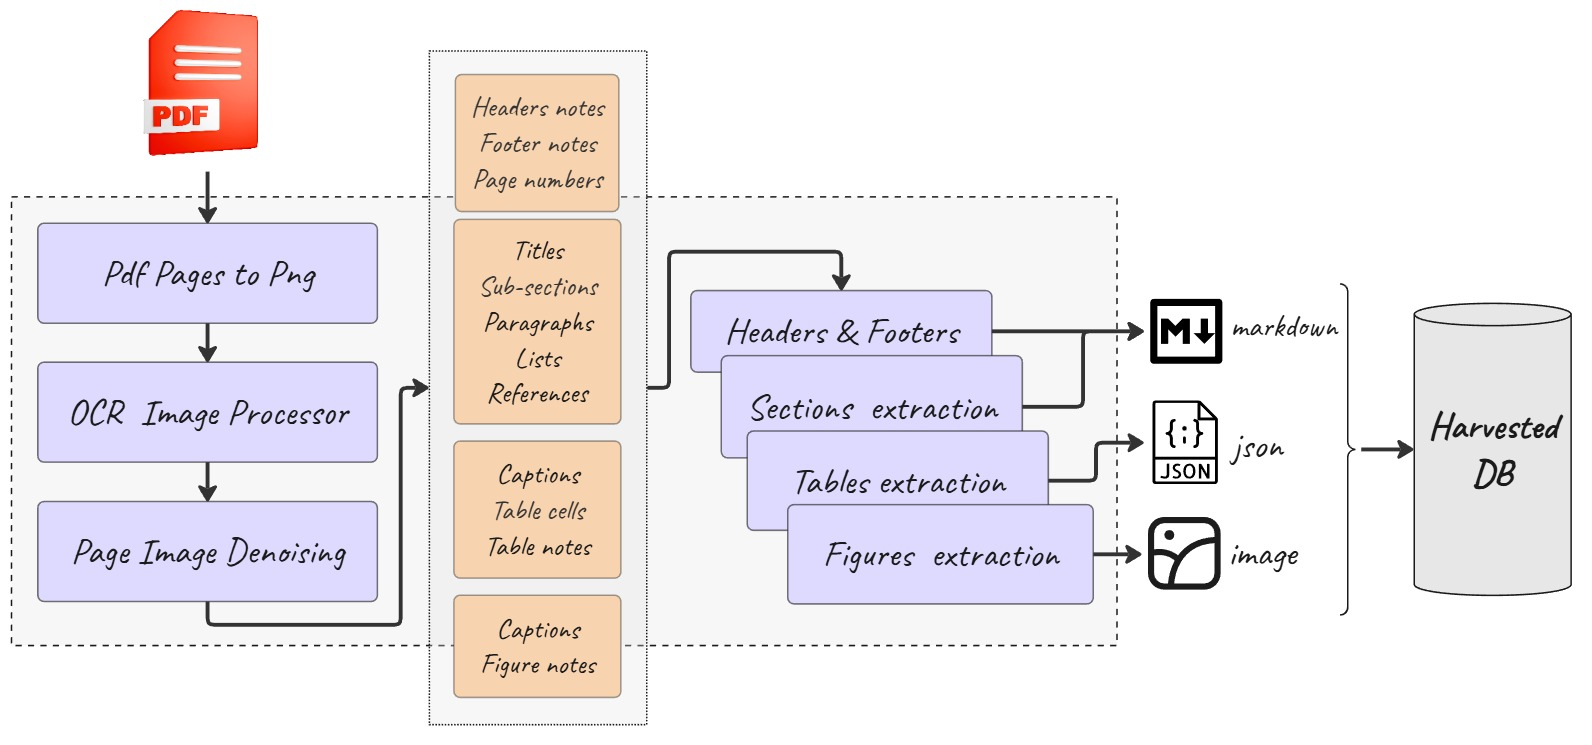
\includegraphics[width=0.7\linewidth]{figures/data_extraction.jpg}
    % \captionsetup{font=footnotesize}
    \caption{Data harvesting workflow. Source documents are processed via OCR, structurally segmented (sections, tables, figures), and stored with provenance in the Harvested database.}
    \label{fig:harvesting_pipeline}
\end{figure}

% Temporary Database (Session Assembly Layer)
During reasoning, strategy plans often require intermediate aggregation, filtering, or transformation of data that should not modify the persistent knowledge base. For this purpose, the framework constructs a temporary, session-scoped database at the start of each control-loop instance. This store is used to hold:
(a) intermediate subsets produced by search or filtering agents,
(b) normalised or reformatted values required for downstream validation,
(c) assembled evidence packets combining multiple knowledge sources, and
(d) transient artefacts generated during multi-step strategies.
The temporary database is strictly short-lived: its contents exist only for the duration of the reasoning episode and are fully captured through the RCP as run-time artefacts. This design ensures that every intermediate transformation remains traceable while preventing contamination of the canonical extracted data.


%==============================================================================
\subsection{Relational Control Plane}
\label{subsec:relational_control_plane}
% \textcolor{red}{Relational Control Plane}
%==============================================================================

The Relational Control Plane (RCP) serves as the central orchestration database of the proposed framework, externalizing coordination logic from code into a normalized relational schema. It provides a generic and auditable foundation for agentic reasoning, particularly within engineering domains where precision, traceability, and validation are essential. Conceptually, the RCP enforces a clear separation between design-time policy and run-time execution. At design time, the library tables define the system’s capability space—strategies are represented as reusable plan templates, while functions are modeled as atomic operations with declared input–output contracts. At run time, corresponding instance tables record each concrete goal, strategy, and function invocation, including their parameters, outputs, validation outcomes, and diagnostic messages. This design allows behaviour to be authored once and reused across multiple domains, while also transforming orchestration into persistent, versioned data that can be Analysed and refined without modifying the underlying control graph.
%%%%%%%%%%%%%%%%%%%%%%%%%%%%%%%%%%%%%%%%%%%%%%%%%%%%%%%%%%%%%%%%%%%%%%%

% [htbp]
\begin{figure*}[!htbp]
    \centering
    % Use [c] alignment to vertically center both elements
    \begin{minipage}[c]{0.38\textwidth}
        \vspace{0pt}
        \centering
        \includegraphics[width=\linewidth]{figures/agentic_flowchart.jpg}
        % Make caption smaller with \small or \footnotesize
        \caption{Agentic control loop showing stages 1--6: iterative goal, strategy, 
        and validation stages interact with persistent and temporary databases to 
        produce a validated result.}
        \label{fig:agentic_flowchart}
    \end{minipage}%
    \hspace{0.03\textwidth} % Controlled spacing instead of \hfill
    \begin{minipage}[c]{0.55\textwidth} % Slightly reduced to accommodate spacing
        % No box - just the algorithm directly
        \vspace{0pt}
        \begin{algorithm}[H]
        \caption{Agentic Reasoning Loop}
        \label{alg:rcp_loop}
        \small
        % \footnotesize
            \begin{algorithmic}[1]
            \definecolor{linecolor}{RGB}{100,100,100}
            \renewcommand{\alglinenumber}[1]{\color{linecolor}\footnotesize #1:}
            
            \State \textbf{Input:} User Query $Q$, Strategy Library $L_S$, Function Library $L_F$
            \State \textbf{Output:} Validated Answer $A$ or Failure Reason $E$
            \State \textbf{Validation:} ValidateFunction (per-step), ValidateStrategy (plan-level), ValidateGoal (final acceptance)
            \State
            \State \textbf{Stage 1: Goal definition} \label{alg:stage1}
            \State $G \gets \text{Normalize}(Q)$ \Comment{Determine targets, evidence granularity, \& validation rules}
            \State $\text{RCP.\,LogGoal}(G)$
            \State
            \State \textbf{Stage 2: Strategy selection} \label{alg:stage2}
            \State $S \gets L_S.\text{FindBestMatch}(G)$ \Comment{Select plan template from Policy Tables}
            \State $\text{RCP.\,LogStrategy}(S)$
            \State
            \State \textbf{Stage 3: Execution loop} \label{alg:stage3}
            \State $P \gets S.\text{PlanSteps}$
            \For{each $Step \in P$}
                \State $f \gets L_F.\text{GetFunction}(Step.\text{Capability})$
                \State $O \gets f.\text{Execute}(Step.\text{Inputs})$
                \State $\text{RCP.\,LogExecution}(f, O)$
                % \State
                \State \textbf{Stage 4: Function validation} \label{alg:stage4}
                \If{$\neg \text{ValidateFunction}(O)$}
                    \State \textbf{retry} $Step$ with adjusted parameters or \textbf{break} to fallback
                \EndIf
                % \State
                \State \textbf{Stage 5: Strategy validation} \label{alg:stage5}
                \If{$\text{ValidateStrategy}(S, O)$}
                    \State \textbf{break} \Comment{Sufficiency criteria met early}
                \EndIf
            \EndFor
            \State
            \State \textbf{Stage 6: Goal validation} \label{alg:stage6}
            \If{$\text{ValidateGoal}(G, S.\text{FinalOutput})$}
                \State \Return $A \gets S.\text{FinalOutput}$
            \Else
                \State \textbf{backtrack} to Stage~2 with broader strategy or \Return $E \gets \text{``No valid strategy''}$
            \EndIf
            \end{algorithmic}
        \end{algorithm}
    \end{minipage}
\end{figure*}
%%%%%%%%%%%%%%%%%%%%%%%%%%%%%%%%%%%%%%%%%%%%%%%%%%%%%%%%%%%%%%%%%%%%%%%%%%%%%
Upon receiving a query, the controller instantiates a goal record with explicit success criteria—such as revision scope, evidence granularity, or citation requirements—and selects an appropriate strategy instance according to stored policies in the RCP libraries.

The controller then dynamically dispatches one or more agents whose input–output contracts match the current system state. Typed contracts are enforced directly within the RCP: each function template defines its expected schema and post-conditions, while validation outcomes at the function, strategy, and goal levels are persisted as structured records in the instance tables. Progress through the loop is therefore validation-centric, with advancement permitted only when defined predicates—such as unit normalization, revision applicability, or citation exactness—are satisfied. All computational artifacts (including structured tables, retrieved passages, intermediate results, and evidence links) are stored within the RCP, whereas the orchestration graph itself maintains only lightweight references, such as the active goal, strategy, or function identifiers. This arrangement minimizes in-memory state, enables reproducible runs, and provides complete observability through standard relational queries.

Compared to conventional agentic frameworks—including standard LangGraph deployments in which logic and execution order are often hard-coded—the RCP introduces three fundamental advances. 
\begin{enumerate}
    \item Changes in execution order, eligibility, or capability preference (for example, inserting a lineage-checking step before finalization or prioritizing hierarchical retrieval over keyword search) are achieved through updates to policy data rather than through code rewrites.
    \item Every decision, artifact, and validation outcome is recorded, enabling deterministic replay, post hoc analysis, and quantitative evaluation of strategy performance.   
    \item New capabilities or alternative implementations (e.g., retrievers, table parsers, or unit normalization tools) can be added by simply registering them within the RCP library, allowing existing strategies to incorporate them immediately without altering the orchestration graph.
\end{enumerate}

Collectively, these properties deliver provenance and audibility by design, while significantly lowering the cost of adapting the framework across domains and document types.

The novelty of the proposed framework lies in its treatment of orchestration as data. Strategies, agent contracts, and validation rules are elevated to persistent, queryable entities within the RCP, while the graph controller functions primarily as an interpreter of these declarative policies. The RCP enables data-driven policy updates rather than architectural redesigns, providing a foundation of generality, audibility, and adaptability that current agentic frameworks lack.
% \subsection{Formalized Reasoning Algorithm}
Algorithm~\ref{alg:rcp_loop} provides the formal pseudocode description of this method.

%==============================================================================
\subsection{Strategy Library}
\label{subsec:strategy_library}
% \textcolor{red}{Strategy Library}
%==============================================================================

The Strategy Library contains reusable plan templates that standardize patterns of tool usage, reasoning, and validation across engineering contexts. Each strategy specifies four core components:
\begin{itemize}[label=- ]
    \item \text{Targets:} The evidence or variables required for successful completion (e.g., numerical value with units, revision identifier, document citation).
    \item \text{Eligible functions:} The permissible computational modules and their preferred execution order (e.g., search → parse → normalize → verify).
    \item \text{Sufficiency conditions:} The coverage and consistency requirements for completion (e.g., two corroborating sources, explicit revision supersession).
    \item \text{Fallback policies:} Adaptive behaviors when sufficiency is not met (e.g., expand search scope, trigger hierarchical retrieval).
\end{itemize}
Concrete instantiations for each case study are presented in Sections~\ref{subsec:hydroscand_case} and~\ref{subsec:saab_case}.


%==============================================================================
\subsection{Function Library}
\label{subsec:function_library}
% \textcolor{red}{Function Library}
%==============================================================================

The Function Library contains modular, atomic operations that execute the steps defined in strategy plans. Each function is a self-contained, side-effect-free component with declared inputs, outputs, and postconditions. Functions compose dynamically to fulfill strategy steps without modifying the orchestration graph, ensuring modularity and maintainability.

Typical functions include: text retrieval (keyword/semantic search with constraint support), hierarchical retrieval (document tree traversal), table extraction (region detection with cell anchoring), unit normalization (canonical conversion with provenance), revision checking (supersession tracing), figure linking, keyword expansion, table filtering, and evidence scoring.

Each function produces validated artifacts (values, units, revisions, citations) that feed into a strategy's target set. Validation gates determine whether these artifacts satisfy sufficiency conditions. When unmet, the orchestration layer invokes additional or alternative functions. Because all functions adhere to uniform interface specifications, components can be replaced without modifying orchestration logic, ensuring interoperability and adaptability across engineering domains.

%==============================================================================
\subsection{In-Session Instantiation}
\label{subsec:in-session_instantiation}
% \textcolor{red}{In-Session Instantiation}
%==============================================================================

Section~\ref{subsec:relational_control_plane} introduced the RCP schema. At runtime, design-time templates are instantiated as session-scoped records. For every user query, the controller creates a goal instance with explicit acceptance criteria and then materializes a strategy instance selected from the Strategy Library. Within this strategy context, the controller dynamically instantiates one or more functions from the Function Library. Each instantiation records its parametrization, inputs consumed, outputs produced, and the results of function-, strategy-, and goal-level validations.
\begin{figure}[!htbp]
    \centering
    \includegraphics[width=0.7\linewidth]{figures/in-session_instantiation_in_RCP3.jpg}
    \caption{RCP relational schema. Design-time library tables (left) define the system’s capability space; run-time session tables (right) record each concrete invocation. Foreign keys (→) enforce the goal → strategy → function hierarchy}
    \label{fig:placeholder_image_insession}
\end{figure}
The in-session tables thus serve as a normalized execution ledger. Inputs and outputs are stored as first-class artifacts linked to their originating strategy and agent instances, together with citations, revision lineage, unit normalizations, and diagnostic messages. The orchestration graph maintains only stable identifiers (e.g., current goal, strategy, and function IDs), while all heavy artifacts—retrieved passages, structured tables with cell anchors, intermediate calculations, and validation reports—reside in the RCP. This arrangement enables deterministic replay and post hoc inspection, supports fine-grained provenance from final answers back to specific clauses or table cells, and provides a coherent basis for evaluation and governance. Because the controller reads policies from the libraries and writes outcomes to the in-session ledger, behaviour can be adapted by updating library entries rather than rewriting orchestration logic. New strategies or functions become immediately available for instantiation once registered, and their inputs/outputs are automatically captured under the same schema. In effect, the RCP operationalizes a data-driven “goal → strategy → agent → validation” loop: strategies and functions defined in the libraries are realized as concrete, auditable instances, and all inputs, outputs, and validations are persistently recorded, ensuring consistent state management and traceable multi-agent reasoning across domains.

%==============================================================================
\subsection{Strategy Selection and System Characteristics}
\label{subsec:strategy_selection_characteristics}
% \textcolor{red}{Strategy Selection and System Characteristics}
%==============================================================================

\subsubsection{Strategy Selection Mechanism}
\label{subsubsec:strategy_selection}

% The controller selects strategies through a rule-based matching algorithm that evaluates goal attributes against strategy preconditions. Strategy templates in the Strategy Library declare eligibility criteria as structured predicates over goal features:
% \begin{itemize}[label=-]
%     \item \text{Entity recognition:} Does the query contain a component identifier?
%     \item \text{Attribute type:} Is the target a simple lookup (single value), comparison (multiple entities), or aggregation (product family) etc.?
%     \item \text{Evidence requirements:} Does the goal require revision awareness, cross-document reasoning, or multimodal synthesis?
%     \item \text{Data availability:} Are authoritative documents, sections or paragraph references identified, or is exploratory search required?
% \end{itemize}

% \noindent The matching algorithm iterates through strategy templates in priority order (defined in \texttt{StrategyLibrary.Priority}), evaluating each template's preconditions against the goal instance. The first strategy whose preconditions are satisfied is selected and instantiated. If no strategy matches, the controller defaults to a generic exploratory strategy or returns a failure diagnostic.
% This rule-based approach ensures deterministic, auditable strategy selection while remaining extensible: new strategies are added by registering templates with appropriate preconditions, requiring no changes to the matching algorithm itself.\\

The controller selects strategies through an LLM-guided evaluation. Upon instantiating a goal, the controller presents the LLM with the current query, a structured goal description, and the ordered list of available strategy templates (excluding those already attempted in the current session). The LLM is prompted to select the most appropriate strategy based on the following criteria:
\begin{itemize}[label=-]
    \item \text{Entity recognition:} Does the query contain a component or product identifier?
    \item \text{Attribute type:} Is the target a simple lookup (single value), comparison (multiple entities), or aggregation (product family)?
    \item \text{Evidence requirements:} Does the goal require revision awareness, cross-document reasoning, or multimodal synthesis?
    \item \text{Data availability:} Are authoritative documents, sections, or paragraph references identified, or is exploratory search required?
\end{itemize}

\noindent The LLM returns a single strategy name drawn from the available list; the selection and its accompanying rationale are persisted to the RCP as a structured record, providing an auditable account of each selection decision. If no valid strategy is returned after retries, the controller falls back to a generic exploratory strategy or returns a failure diagnostic. Because selection criteria are embedded in the prompt rather than in hard-coded predicates, new strategies are registered by adding a named template to the Strategy Library—no changes to the controller are required.

Note that the current LLM-guided selection approach, while traceable, introduces a degree of non-determinism at the selection step. A planned code-level enhancement will replace this with a structured, rule-based precondition matching mechanism—where each strategy template explicitly declares eligibility predicates over goal features—making strategy selection fully deterministic and auditable independently of any LLM call.\\
% \begin{figure}[t]
% \centering
% \includegraphics[width=0.85\linewidth]{figures/strategy_selection_flow.png}
% \caption{Illustration of the rule-based strategy selection process. Query-derived goal features are evaluated against strategy template predicates. The first template whose preconditions are satisfied is selected and instantiated for execution.}
% \label{fig:strategy_selection}
% \end{figure}

% \subsubsection{Computational Characteristics}
% \label{subsubsec:computational_characteristics}

% \textbf{Time complexity:} Strategy selection is $O(S \cdot P)$, where $S$ is the number of strategy templates and $P$ is the average number of precondition checks per template. In practice, $S < 20$ for domain-specific instantiations, making selection overhead negligible compared to function execution costs (retrieval, parsing, LLM inference).

% Function execution time is dominated by external operations: database queries ($O(\log N)$ to $O(N)$ for full-text search over $N$ documents), table parsing ($O(T \cdot R \cdot C)$ for $T$ tables with $R$ rows and $C$ columns), and LLM inference ($O(L)$ where $L$ is context length, typically 2K--8K tokens per call).

% \textbf{Space complexity:} The RCP stores all orchestration artifacts as relational records. For a session with $G$ goals, $S$ strategy instances, and $F$ function calls, storage is $O(G + S + F \cdot (I + O))$, where $I$ and $O$ are average input and output sizes per function. Typical sessions generate 10--50 function calls with aggregate storage under 1~MB per query.

% \textbf{Latency characteristics:} End-to-end latency ranges from 2--15 seconds for simple lookups (1--3 function calls) to 30--90 seconds for complex multi-document reasoning (10--20 function calls). Parallel execution (Case~II, Strategy~3) reduces latency by 30--50\% when independent function calls are identified.

% \subsubsection{Limitations and Applicability}
% \label{subsubsec:limitations}

% The proposed framework is designed for engineering document reasoning where \textbf{validation, traceability, and determinism} are critical. It is \textbf{not appropriate} for:

% \begin{itemize}
%     \item \textbf{Open-ended creative generation:} The validation-centric architecture enforces evidence grounding, limiting unconstrained text generation.
%     \item \textbf{Real-time, low-latency applications:} RCP persistence and multi-stage validation introduce overhead unsuitable for sub-second response requirements.
%     \item \textbf{Domains with sparse or unstructured knowledge bases:} The framework assumes a harvested, structured knowledge layer; it does not perform well on raw, unprocessed corpora.
%     \item \textbf{Single-shot, stateless queries:} The orchestration overhead is unjustified when a single retrieval + generation step suffices.
% \end{itemize}

% \textbf{Current limitations include:}

% \begin{itemize}
%     \item \textbf{Manual strategy authoring:} Strategy templates are currently hand-crafted for each domain. Automatic strategy synthesis from example queries remains future work.
%     \item \textbf{Limited cross-session learning:} The framework does not currently adapt strategy selection or function parameters based on historical execution outcomes.
%     \item \textbf{Scalability of in-session storage:} Very long reasoning chains (50+ function calls) may exceed practical in-session storage limits, requiring garbage collection or summarization.
%     \item \textbf{Dependency on structured extraction quality:} The framework's reliability depends on the quality of the harvested knowledge base. Errors in document parsing propagate to downstream reasoning.
% \end{itemize}

% Despite these limitations, the framework demonstrates significant advantages in domains where multi-step reasoning, rigorous validation, and complete auditability are essential—characteristics that define engineering knowledge work.


% ###################################################### ADDED

% ===============================================================
% DOMAIN APPLICATION
% ===============================================================
\section{Domain Application}
\label{sec:domain_application}

This section presents two industrial applications used to evaluate the proposed framework. We describe the domain-specific instantiation choices, including document harvesting design, strategy and function libraries, and validation-flow configuration. Representative execution traces illustrate how validation gates limit unsupported claims and how the RCP enables inspection of intermediate artifacts. A full quantitative evaluation is provided in Section~\ref{sec:evaluation}.

Case~I (Hydroscand) addresses catalogue-style extraction from dense, multilingual tables with typographic variation. Case~II (SAAB) evaluates query-driven reasoning over revision-controlled engineering documents with heterogeneous layouts and applicability constraints. For each case, we describe the instantiation process, and present representative execution traces.


\subsection{CASE I: Industrial Hydraulic Products Catalog (Hydroscand AB)}
\label{subsec:hydroscand_case}
\noindent Industrial hydraulic systems rely on extensive product catalogues that consolidate specifications for hoses, fittings, and coupling assemblies. These multi-page documents encode critical attributes such as dimensions, pressure ratings, reinforcement structures, material compositions, thread standards etc. The Hydraulic Produktbok \cite{hydroscand2020produktbok}, a widely used Nordic fluid-power reference from Hydroscand AB, a leading provider of hydraulic and industrial hose solutions, is representative of this class: it presents chapter-organised product families, construction descriptions, and dense specification tables spanning numerous variants within each product line.

The catalogue’s structure poses notable challenges for automated knowledge extraction. Variant-level data appear in compact tables with merged cells, multi-row headers, mixed unit conventions, and visually implied hierarchies. Thread standards (BSP/G, JIC, ORFS, NPTF) depend on subtle typographic distinctions that OCR and naive PDF parsers often distort. Free-text descriptions (entirely in Swedish) use specialised terminology that impede generic retrieval models. Consequently, conventional approaches such as keyword search or chunk-based RAG tend to lose table semantics, misinterpret values, or fail to deliver cell-level, engineering-grade citations. General-purpose retrievers also lack the domain grounding needed for queries based on technical specifications, such as pressure-rating lookup, thread-compatibility checks or application-based product selection.

% reason for choosing this domain
This environment thus presents an appropriate proof-of-concept domain for the proposed framework. It combines heterogeneous modalities (tables, free text, mixed typography), domain-specific naming conventions, and a need for strict validation of engineering attributes. Successfully demonstrating reliable extraction and reasoning here directly tests the framework’s ability to mitigate hallucination, preserve unit fidelity, and deliver verifiable outputs with explicit provenance.

To operationalize extraction and reasoning, the framework is instantiated through a layered architecture that separates document processing, agent orchestration, and application-level interaction.

%_______________________________________________________________________________
\subsubsection{Layer 1: Document Pre-processing/Extraction (Case I)}
\label{subsubsec:Extraction Pipeline}

The extraction layer converts source documents into a normalized relational database (harvested.db). Each page is rendered at high resolution to preserve typographic fidelity—critical for distinguishing notation spacing (e.g., "G 1/2" vs. "G1/2"), sub/superscripts, and unit annotations that carry semantic meaning.
\begin{figure}[!htbp]
    \centering
    \includegraphics[width=0.9\linewidth]{figures/press_coupling.jpg}
    \caption{Sample data extraction from a product category (Press coupling)}
    \label{fig:placeholder_image1}
\end{figure}
% Objectification for storage
Parsed content are inserted into a relational schema: \textit{categories} (e.g., Högtrycksslang, Presskopplingar), \textit{families} (e.g., Kappaflex 2K, T9090) and \textit{product-level variants} (e.g., 1105-10-04, 1059-00-16)
The objective here is not merely to extract product data, but to reconstruct the catalogue’s implicit structure: the hierarchical organisation of categories and product families, the fine-grained geometry of specification tables, and the contextual metadata that defines material properties, thread standards, and operating limits. By decoupling extraction from reasoning, the system ensures that all downstream tasks operate on validated, structured data rather than raw PDF content.

%_______________________________________________________________________________
\subsubsection{Layer 2: Agentic Reasoning (Case~I)}
\label{subsubsec:Agentic Reasoning}

The agentic reasoning layer operationalises the six-stage control loop described in Section~\ref{subsec:relational_control_plane}. A user query (e.g., specification lookup,compatibility assessment, or family-level aggregation) is normalised into a structured \textit{goal instance} with explicit evidence requirements (target attribute, value type, and validation predicate).The controller then selects an appropriate \textit{strategy instance} and executes an ordered \textit{function plan}. All orchestration artifacts—including goal, strategy selection, function invocations, inputs, outputs, and validation outcomes—are persisted in the relational control plane (\texttt{agentic.db}), enabling replay, inspection, and failure attribution at record level.

While Section~\ref{subsec:relational_control_plane} --\ref{subsec:in-session_instantiation} define the generic control loop and RCP schema, this section focuses on their concrete instantiation for catalogue-based reasoning. All described artifacts correspond to rows in the relational control plane and are not conceptual abstractions.\\

%Implementation
\noindent {\textbf{Strategy templates:}}
Product catalogue queries exhibit a small number of recurring patterns. In this case study, most requests fall into four archetypes: (i) direct specification lookup for a known product code, (ii) contextual search with attribute constraints, (iii) compatibility checks between components, and (iv) aggregation across product families. These archetypes are encoded as declarative strategy templates in the \texttt{StrategyLibrary} table, each specifying a target, an ordered plan skeleton, and a sufficiency condition that determines whether the goal is satisfied. Table~\ref{tab:strategy_templates} summarises an exemplary strategy set instantiated for the catalogue domain.\\

% ============================================
% TABLE: Strategy Templates for Case I
% ============================================
\begin{table*}[!htbp]
\captionsetup{width=0.92\linewidth, skip=2pt}
    \caption{Strategy templates for hydraulic catalogue queries.}
    \label{tab:strategy_templates}
    \centering
    \small
    \setlength{\tabcolsep}{6pt}
    \renewcommand{\arraystretch}{1}
    \begin{tabularx}{\textwidth}{c p{1.9cm} X p{4.5cm} p{2.8cm}}
    \toprule
    \textbf{ID} &
    \textbf{Strategy} &
    \textbf{Description} &
    \textbf{Plan steps} &
    \textbf{Suff. condition} \\
    
    \midrule
    
    1 & 
    \textit{Specification Lookup} &
    Retrieve a known specification from an identified product code. &
    Extract product code $\rightarrow$ Query database $\rightarrow$ Extract attributes $\rightarrow$ Analyze with LLM &
    Attribute found and unit normalized. \\
    
    \midrule
    
    2 &
    \textit{Contextual Product Search} &
    Identify candidate products matching textual or semantic constraints. &
    Extract requirements $\rightarrow$ Semantic search $\rightarrow$ Filter items $\rightarrow$ Extract attributes $\rightarrow$ Analyze with LLM &
    At least one valid product returned. \\
    
    \midrule
    
    3 &
    \textit{Compatibility Check} &
    Assess coupling or thread compatibility between two hydraulic components. &
    Extract component specifications $\rightarrow$ Match standards $\rightarrow$ Check dimensional compatibility $\rightarrow$ Analyze with LLM &
    Standards matched; no dimensional conflict. \\
    
    \midrule
    
    4 &
    {\textit{Family Summary}} &
    Aggregate specification data across all variants within a product family. &
    Retrieve family variants $\rightarrow$ Extract attributes $\rightarrow$ Aggregate results $\rightarrow$ Analyze with LLM &
    Full variant set retrieved and schema consistent. \\
    
    \bottomrule
    \end{tabularx}
\end{table*}

%_______________________________________________________________________________
\noindent \textbf{Function Library:} Functions are atomic capabilities that populate strategy plans. In this implementation, functions are exposed through a standard interface (\texttt{success: bool, result: dict}) and are registered in the \texttt{Function Library} with declared inputs, outputs, and postconditions. Table~\ref{tab:agent_functions_hydraulic_catalog} lists the core function set used in the hydraulic catalogue case.

\begin{table*}[!htbp]
\captionsetup{width=0.92\linewidth, skip=2pt}
    \caption{Function library for the hydraulic catalogue domain.}
    \label{tab:agent_functions_hydraulic_catalog}
    \centering
    \small
    \setlength{\tabcolsep}{5pt}
    \renewcommand{\arraystretch}{1}
    \begin{tabularx}{\textwidth}{c >{\raggedright\arraybackslash}p{4cm} p{5.8cm} X}
    \toprule
    \textbf{ID} & 
    \textbf{Function Name} & 
    \textbf{Purpose} &
    \textbf{Artifact Produced} \\
    \midrule
    
    1 & \textit{func\_extract\_products} &
    Retrieve candidate products using keywords and filters. &
    List of product codes with summary specifications. \\
    
    \midrule
    
    2 & \textit{func\_filter\_by\_attribute} &
    Narrow a product list by applying attribute constraints (e.g., pressure, DN size). &
    Filtered list satisfying the specified constraints. \\
    
    \midrule
    
    3 & \textit{func\_get\_product\_details} &
    Retrieve complete specifications and provenance for a given product. &
    JSON object with metadata and catalog page reference. \\
    
    \midrule
    
    4 & \textit{func\_extract\_attributes} &
    Extract target attribute values from a product specification. &
    Attribute values with units and citations. \\
    
    \midrule
    
    5 & \textit{func\_normalize\_units} &
    Convert values to canonical units while preserving original formats. &
    \(420\,\text{bar} \rightarrow 42\,\text{MPa}\). \\
    
    \midrule
    
    6 & \textit{func\_analyse\_data} &
    Compose the final answer with citations and verified source trace. &
    Grounded explanation linked to catalog data. \\
    
    \midrule
    
    7 & \textit{func\_extract\_product\_code} &
    Identify and validate a product identifier from a free-text query. &
    Validated product code (e.g., 4201-16-16). \\
    
    \bottomrule
    \end{tabularx}
\end{table*}
%_______________________________________________________________________________

Notably, \textit{func\_analyse\_data}\footnote{For clarity, human-readable function labels (e.g., Analyse With LLM, etc.) are mapped internally to registered callable identifiers (e.g., \texttt{func\_analyse\_data}) defined in the Function Library.} performs a structured LLM synthesis over verified intermediate artifacts. It is instructed to preserve catalogue terminology (e.g., “Arbetstryck”, “Gängtyp”), avoid unsupported claims, and reference source-provenance fields. All other functions operate deterministically over structured records (from \texttt{harvested.db}), enabling validation gates to intercept failures before an answer is returned.

These functions adhere to a standardized interface (success: bool, result: dict), enabling orchestration via LangGraph without bespoke code. As a result, adding new capabilities (e.g., func\_check\_temperature\_range) involves no orchestration modification—only policy entry registration.

%_______________________________________________________________________________
\subsubsection{Layer 3: Application-level interaction (Case I)}
\label{subsubsec:Application-level interaction}
The application layer exposes the reasoning system through a Flask-Based Web Interface. It offers an interactive front-end tailored for exploratory use and inspection. It accepts free-form queries, which are normalized and submitted to the controller as goal instances. The interface provides real-time visualizations of the reasoning process, including progress through strategy stages, intermediate agent outputs, and final structured answers. Crucially, all responses are enriched with provenance annotations: source, page numbers, and references presented alongside normalized attributes to preserve interpretability.

%_______________________________________________________________________________
\subsubsection{{Worked Example: End-to-End Execution (Case I)}}
\label{subsubsec:worked_example_case_I}

To illustrate end-to-end behaviour, this subsection traces a representative specification query:
\begin{quote}
    \centering
    \emph{``\textbf{Vilken gängstorlek har en 4201-16-16?}''} \\
    (\textit{``What is the thread size of 4201-16-16?''})
\end{quote}

\noindent The system must:
    \textbf{(i)} recognise the product code, 
    \textbf{(ii)} retrieve the corresponding catalogue record, 
    \textbf{(iii)} extract the requested attribute (thread size), and 
    \textbf{(iv)} generate a grounded response. 
Although the query is simple, it exercises the framework’s defining elements: explicit separation of goals, strategies, and functions, and validation gates that prevent incomplete or unsupported answers.\\

%______________________________________________________________________________________________________
\noindent \textbf{Goal definition:}
Execution begins at \texttt{GoalDefine}, where the free-text query is normalised into a structured goal instance with explicit evidence requirements. An LLM extracts key entities (product: ``4201-16-16''; attribute: ``gängstorlek'') and the controller writes a new record to \texttt{GoalInSession}. The goal specifies the target type (product specification) and a validation predicate requiring that the thread-size attribute is resolved for the identified product before the session can be marked successful (Table~\ref{tab:worked_example_goal}).

This goal record is the trace anchor: all subsequent strategy and function records reference \texttt{Goal\-ID} either directly (strategy) or transitively (functions via \texttt{Strategy\-ID}).\\

%______________________________________________________________________________________________________
\noindent \textbf{Strategy selection:}
Control transitions to the \texttt{Strategy\-Plan} node, where the goal instance is matched against \texttt{StrategyLibrary}. Because the query contains an explicit high-confidence product identifier, the controller selects \textit{Specification Lookup} rather than broader retrieval strategies. The resulting strategy instance, including an ordered plan (\texttt{PlanSteps}) and sufficiency condition, is persisted to \texttt{Strategy\-In\-Session} (Table~\ref{tab:strategy_instance_table}).

\begin{table}[!htbp]
\captionsetup{width=0.95\linewidth, skip=5pt}
\caption{Goal and strategy instances for the worked example (Case I).}
\label{tab:goal_strategy_sidebyside}
\centering
\small
\setlength{\tabcolsep}{2pt}
\renewcommand{\arraystretch}{1.0}
\subcaptionsetup{skip=0.5pt}
\subcaptionbox{Goal instance.\label{tab:worked_example_goal}}[0.49\linewidth]{
\begin{tabular}{@{}p{0.32\linewidth}@{\hspace{2pt}}p{0.64\linewidth}@{}}
\toprule
\textbf{Field} & \textbf{Value} \\
\midrule
GoalID & \texttt{1} \\
SessionID & \texttt{083} \\
GoalName & \texttt{Main goal} \\
Target & \texttt{Product specification} \\
Validation & \texttt{Thread size resolved for identified product} \\
Description & \texttt{Determine the standard thread size of a 4201-16-16 coupling} \\
GoalSuccess & \texttt{NULL} \\
\bottomrule
\end{tabular}
}
\hfill
\subcaptionbox{Strategy instance.\label{tab:strategy_instance_table}}[0.49\linewidth]{
\begin{tabular}{@{}p{0.34\linewidth}@{\hspace{3pt}}p{0.60\linewidth}@{}}
\toprule
\textbf{Field} & \textbf{Value} \\
\midrule
StrategyID & \texttt{1} \\
GoalID & \texttt{1} \\
StrategyName & \texttt{Specification Lookup} \\
Target & \texttt{Product specification} \\
Description & \texttt{Direct lookup of a known specification from an identified product code} \\
PlanSteps & \texttt{Extract product code; retrieve product details; extract attributes; analyse with LLM} \\
Sufficiency & \texttt{Attribute found and unit normalized} \\
StrategySuccess & \texttt{NULL} \\
\bottomrule
\end{tabular}
}
\end{table}

\noindent This provides explicit, auditable linkage between the abstract strategy template and the executable sequence, yielding a compact, query-specific "recipe" that can be replayed or inspected independently.\\
%_________________________________________________________________________________

\noindent \textbf{Function execution \& validation:}
Execution proceeds to \texttt{FunctionExecute}, which iterates deterministically over the ordered \texttt{PlanSteps}. For each step, the invocation is recorded in \texttt{FunctionInSession}, while inputs and outputs are materialised as key--value records in \texttt{FunctionParametersInSession} and \texttt{FunctionOutputInSession}. After each call, \texttt{FunctionValidate} enforces basic correctness (e.g., non-empty outputs, expected keys present, count $>$ 0), preventing the plan from advancing when a prerequisite artifact is missing.\\
For readability, Tables~\ref{tab:worked_example_func1}--\ref{tab:worked_example_func4} present compact projections of the corresponding in-session function, parameter, and output records.

%_______________________________________________________________________________
\begin{enumerate}[label=\roman*, itemsep=8pt]
    \item {\textit{Function 1} – Extract Product Number:}
    The first function processes the query string and extracts the product code (``4201-16-16'') for downstream lookup. The output is stored as a structured parameter (e.g., keyword output = ``4201-16-16''), and the function is marked successful. This isolates the product identifier in a form suitable for database lookup.
        (Table~\ref{tab:worked_example_func1}.)
       
    \item {\textit{Function 2} – Query Database:}
        The second function constructs a SQL query against the harvested product table, using "keyword output" as key. It returns a structured product record, including a specification field (e.g., a JSON or key--value map), and writes both the raw result and a count field to the function output store. Validation at this point requires count $>$ 0; an empty result would immediately fail the strategy and route control to Strategy\-Validate. 
        (Table~\ref{tab:worked_example_func2}.)
    
    \item {\textit{Function 3} – Extract Attributes:}
        The third function operates on the retrieved record and projects out the requested attribute. It extracts the \textit{gängstorlek} field (e.g., G1) from the specification structure and stores it as Extracted Attributes. Validation checks that the requested key is present and that its value is non-empty. Failure here would prevent the LLM from synthesizing an answer that satisfies the goal predicate.
        (Table~\ref{tab:worked_example_func3}.)
    
    \item {\textit{Function 4} – Analyse With LLM:}
        The final function receives the original query and Extracted Attributes as input. It generates a concise natural-language answer that states the thread size for the identified product, preserving catalogue terminology. The answer text is stored as Analyse Output, and the function is marked successful if the output is non-empty and well-formed.
        (Table~\ref{tab:worked_example_func4}.)
\end{enumerate}

%%%%%%%%%%%%%%%%%%%%%%%%%%%%%%%%%%%%%%%%%%%%%%%%%%%%%%%%%%%%%%%%%%%%%%%%%%%%%%%
\begin{table}[!htbp]
    \captionsetup{width=0.8\linewidth, skip=5pt}
    \caption{Function execution trace.}
    \label{tab:worked_example_grouped}
    \centering
    \small
    \setlength{\tabcolsep}{2pt}
    \renewcommand{\arraystretch}{1.0}
    
    \subcaptionsetup{skip=0.5pt}
    \subcaptionbox{Extract Product Number.\label{tab:worked_example_func1}}[0.49\linewidth]{
    \begin{tabular}{@{}p{0.34\linewidth}@{\hspace{3pt}}p{0.60\linewidth}@{}}
        \toprule \textbf{Field} & \textbf{Value} \\
        \midrule
        FunctionID & \texttt{1} \\
        StrategyID & \texttt{1} \\
        FunctionName & \texttt{func\_extract\_products} \\
        Inputs & \texttt{Query string} \\
        Outputs & \texttt{Keyword Output = 4201-16-16} \\
        ValidationResult & \texttt{Output non-empty; format valid} \\
        FunctionSuccess & \texttt{1} \\
        \bottomrule
    \end{tabular}
    }\hfill
    \subcaptionbox{Query Database.\label{tab:worked_example_func2}}[0.49\linewidth]{
    \begin{tabular}{@{}p{0.34\linewidth}@{\hspace{3pt}}p{0.60\linewidth}@{}}
        \toprule \textbf{Field} & \textbf{Value} \\
        \midrule
        FunctionID & \texttt{2} \\
        StrategyID & \texttt{1} \\
        FunctionName & \texttt{func\_get\_product\_details} \\
        Inputs & \texttt{Keyword Output = 4201-16-16} \\
        Outputs & \texttt{Product record; count = 1} \\
        ValidationResult & \texttt{count $>$ 0; count and format valid} \\
        FunctionSuccess & \texttt{1} \\
        \bottomrule
    \end{tabular}
    }
    
    \vspace{15pt}
    
    \subcaptionbox{Extract Attributes.\label{tab:worked_example_func3}}[0.49\linewidth]{
    \begin{tabular}{@{}p{0.34\linewidth}@{\hspace{3pt}}p{0.60\linewidth}@{}}
        \toprule \textbf{Field} & \textbf{Value} \\
        \midrule
        FunctionID & \texttt{3} \\
        StrategyID & \texttt{1} \\
        FunctionName & \texttt{func\_extract\_attributes} \\
        Inputs & \texttt{Product specification record} \\
        Outputs & \texttt{Extracted attributes: \textit{gängstorlek} = G1"} \\
        ValidationResult & \texttt{Attribute present and non-empty} \\
        FunctionSuccess & \texttt{1} \\
        \bottomrule
    \end{tabular}
    }\hfill
    \subcaptionbox{Analyse with LLM.\label{tab:worked_example_func4}}[0.49\linewidth]{
    \begin{tabular}{@{}p{0.34\linewidth}@{\hspace{3pt}}p{0.60\linewidth}@{}}
        \toprule \textbf{Field} & \textbf{Value} \\
        \midrule
        FunctionID & \texttt{4} \\
        StrategyID & \texttt{1} \\
        FunctionName & \texttt{func\_analyse\_data} \\
        Inputs & \texttt{Query and extracted attributes} \\
        Outputs & \texttt{Natural-language answer stating thread size} \\
        ValidationResult & \texttt{Output non-empty; well-formed} \\
        FunctionSuccess & \texttt{1} \\
        \bottomrule
    \end{tabular}
    }
\end{table}
%_______________________________________________________________________________
% \noindent \textbf{Function parameter and output schemas:}
% Beyond runtime traces, the framework maintains declarative schemas for function inputs and outputs. \texttt{FunctionParametersLibrary} and \texttt{FunctionOutputLibrary} define the expected keys, types, and semantics for each registered function. At execution time, these schemas are used to validate records written to \texttt{FunctionParametersInSession} and \texttt{FunctionOutputInSession}, enabling early detection of malformed inputs, missing fields, or incompatible outputs before downstream functions are invoked.

% Each function invocation results in multiple parameter and output records, materialised as rows in \texttt{FunctionParametersInSession} and \texttt{FunctionOutputInSession}, respectively.\\

% Below excerpt illustrates how each function invocation materialises concrete output artifacts in \texttt{FunctionOutputInSession}, enabling fine-grained inspection, replay, and failure attribution at record level.

\noindent \textbf{Function parameter and output schemas:}
Beyond runtime traces, the framework maintains declarative schemas for function inputs and outputs. \texttt{FunctionParametersLibrary} and \texttt{FunctionOutputLibrary} define the expected keys, types, and semantics for each registered function. At execution time, these schemas validate records written to \texttt{FunctionParametersInSession} and \texttt{FunctionOutputInSession}, enabling early detection of malformed inputs, missing fields, or incompatible outputs before downstream functions are invoked.

Each function invocation results in multiple parameter and output records, materialized as rows in these in-session tables. Complete parameter and output records for this worked example are provided in Appendix~\ref{app:detailed_traces_case1}, demonstrating how each function invocation materializes concrete artifacts enabling fine-grained inspection, replay, and failure attribution at record level.
The combination of \texttt{FunctionExecute} and \texttt{FunctionValidate} therefore yields a linear, record-level trace: each intermediate artifact (product code, retrieved record, extracted attribute, final response) is persisted and linked to the function invocation that produced it.

This worked example demonstrates how goal satisfaction emerges from validated, sequential agent execution, with all intermediate artifacts persisted in the Relational Control Plane (RCP). Only representative parameters are shown; auxiliary configuration fields (e.g., joins, ordering, custom SQL) are omitted for brevity.



% =======================================
% CASE II
% =======================================
\subsection{CASE II: Revision-Controlled Aerospace Documentation \texttt{(Saab AB)}}
\label{subsec:saab_case}

While the first case addressed a somewhat semi-structured product catalogue, this second application focused on query‑driven interaction with a corpus of technical manuals where cross-document consistency and revision fidelity are critical. this case targets yet again, a heterogeneous and multilingual content, applicability constraints, and multimodal layout. This study was conducted in collaboration with Saab AB (Svenska Aeroplan Aktiebolaget) — a leading Swedish aerospace and defense company.   

Engineering documentation in this domain differs fundamentally from the catalog-style product data as in the previous case, requiring reasoning across multiple,multilingual, heterogeneous documents, with relevant information distributed across textual, tabular, and graphical elements. Answering a single query may therefore require coordinated retrieval, structured extraction, and fusion of evidence from several sources. The case hence motivate explicit orchestration of document-level strategies and function-level operations, with persistent execution traces that capture how intermediate artifacts are produced, combined, and verified before a response is returned.

In compliance with confidentiality requirements, proprietary identifiers, document titles, part numbers, and content values shown in this case study have been anonymized or abstracted. The execution traces, schemas, and control logic presented here nevertheless reflect real runtime artifacts persisted within the RCP.

%_______________________________________________________________________________
\subsubsection{Layer 1: Document Pre-processing/Extraction (Case II)}
\label{subsubsec:saab_document_harvesting}

% This case, also underpinned by a harvested, document-centric knowledge database that preserves applicability metadata and structural context at extraction time. Source documentation spans heterogeneous formats and layouts, including narrative requirements, dense tables, and figure-referenced descriptions. During ingestion, each document is represented as linked relational units capturing: (i) document identity and revision markers,(ii) section hierarchy (e.g., headings and paragraphs), and (iii) modality-specific artifacts (text passages, table fragments, and figure-referenced elements).

\textcolor{red}{This case is also underpinned by a harvested, document-centric knowledge database that preserves applicability metadata and structural context at extraction time. The ingested corpus comprises \textbf{54 source documents} yielding \textbf{451 technical tables}, \textbf{576 annotated images}, and \textbf{3,488 text segments}. The domain encompasses six product series spanning electronic connectors, cable assemblies, and filter components, with product codes following multiple format conventions requiring dedicated normalization (e.g., space/dash insertion, prefix handling). Source documentation spans heterogeneous formats and layouts, including narrative requirements, dense tables, and figure-referenced descriptions. During ingestion, each document is represented as linked relational units capturing: (i)~document identity and revision markers, (ii)~section hierarchy, and (iii)~modality-specific artifacts (text passages, table fragments, and figure-referenced elements).}

Extracted records retain anchors such as section labels, table captions, and page references, enabling downstream evidence selection to remain location-aware (clause/table/figure context), not merely content-aware. The harvested representation supports query-time disambiguation when multiple candidate sources coexist (e.g., overlapping documents or revisions) and provides stable evidence units for subsequent goal–strategy–agent execution and validation.

%_______________________________________________________________________________
\subsubsection{Layer 2: Agentic Reasoning (Case II)}
The Case II reuses the same six-stage goal–strategy–agent control loop introduced in Section~\ref{subsec:relational_control_plane}. No architectural modifications were required; instead, the framework is instantiated through a richer set of strategy templates and functions tailored to document-centric reasoning. Compared to the previous case, Case II exercises deeper strategy plans, parallel execution blocks, and multimodal artefacts. The same relational control plane schema governs both cases, further demonstrating the generality of the framework.\\

\noindent \textbf{Strategy templates:}
Table~\ref{tab:saab_strategy_templates} presents strategy templates for this domain. Each template follows the structure defined in Section~\ref{subsec:strategy_library}: targets, eligible functions, sufficiency conditions, and fallback policies.\\


% ============================================
% TABLE: Strategy templates instantiated for case II domain.
% ============================================
\begin{table*}[!htbp]
\captionsetup{width=0.92\linewidth, skip=2pt}
    \caption{Strategy templates instantiated for Case II domain.}
    \label{tab:saab_strategy_templates}
    \centering
    \small
    \setlength{\tabcolsep}{6pt}
    \renewcommand{\arraystretch}{1.1}
    \begin{tabularx}{\textwidth}{c p{2.2cm} X p{5cm} X}
    % \begin{tabularx}{\textwidth}{>{\centering\arraybackslash}p{0.5cm} p{1.5cm} X p{4.2cm} p{3.5cm}}
    
    \toprule
    \textbf{ID} &
    \textbf{Strategy} &
    \textbf{Description} &
    \textbf{PlanSteps} &
    \textbf{Suff. condition} \\
    
    \midrule
    
    1 & \textit{Simple Lookup} &
    Deterministic retrieval of structured information from a single authoritative document. & Extract product code $\rightarrow$ Find latest document $\rightarrow$ Table search
    $\rightarrow$ Filter table $\rightarrow$ Assemble table $\rightarrow$ Analyse with LLM & Requested attribute resolved with supporting evidence. \\
    
    \midrule
    
    2 & \textit{Enhanced Lookup} &
    Multi-stage table reasoning with contextual filtering and aggregation. &
    Extract product code $\rightarrow$ Table search $\rightarrow$ Filter table
    $\rightarrow$ Assemble table $\rightarrow$ Analyse with LLM & Consistent result derived across candidate records. \\
    
    \midrule
    
    3 & \textit{Parallel Enhanced Lookup} &
    Latency-aware strategy executing independent steps concurrently. &
    Extract product code $\rightarrow$ Find latest document $\rightarrow$
    [Table search $\parallel$ Document search]
    $\rightarrow$ Filter table $\rightarrow$
    [Analyse with LLM $\parallel$ Convert units]
    $\rightarrow$ Aggregate results & Requested attribute resolved and validated. \\
    
    \midrule
    
    4 & \textit{Visual Layout Generation} &
    Multimodal retrieval and synthesis of layout-level information. &
    Extract product code $\rightarrow$ Retrieve image asset
    $\rightarrow$ Generate visual layout $\rightarrow$ Analyse with LLM &
    Layout produced and grounded in source document. \\
    
    \bottomrule
    \end{tabularx}
    
    \vspace{2mm}
    \raggedright
    \footnotesize
    \textit{Note:} Parallel steps are indicated with the $\parallel$ symbol.
\end{table*}
%_______________________________________________________________________________

\noindent \textbf{Function library:}
The strategies in Table~\ref{tab:saab_strategy_templates} are instantiated using callable \emph{functions} registered in the \texttt{Function Library}, some are shown in Table~\ref{tab:saab_function_library} for this domain application. In this paper, we use \emph{agent} to denote the reasoning entity that orchestrates the workflow, and \emph{function} to denote the atomic executable operation with a typed input–output contract. This distinction enables deterministic orchestration and schema-level validation. Human-readable labels are used in the narrative, while callable identifiers are shown verbatim in the tables.

%_______________________________________________________________________________
\begin{table*}[!htbp]
\captionsetup{width=0.92\linewidth, skip=2pt}
    \caption{Functions used in the SAAB documentation case.}
    \label{tab:saab_function_library}
    \centering
    \small
    \setlength{\tabcolsep}{5pt}
    \renewcommand{\arraystretch}{1.1}
    \begin{tabularx}{\textwidth}{c >{\raggedright\arraybackslash}p{4.2cm} p{6.0cm} X}
    \toprule
    \textbf{ID} &
    \textbf{Function Name} &
    \textbf{Purpose} &
    \textbf{Artifact Produced} \\
    \midrule
    1 & \textit{func\_extract\_product\_code} &
    Identify and validate a product or component identifier from a free-text query. &
    Validated identifier token. \\
    
    \midrule
    
    2 & \textit{func\_find\_latest\_document} &
    Select the most recent applicable document revision from the corpus. &
    Document surrogate ID. \\
    
    \midrule
    
    3 & \textit{func\_table\_search} &
    Locate candidate tables within a document matching query constraints. &
    Table records and metadata. \\
    
    \midrule
    
    4 & \textit{func\_filter\_table} &
    Apply rule-based and semantic filters to tabular data. &
    Filtered table rows. \\
    
    \midrule
    
    5 & \textit{func\_assemble\_table} &
    Merge and normalize table fragments into a unified structure. &
    Structured table artifact (JSON). \\
    
    \midrule
    
    6 & \textit{func\_generate\_visual\_layout }&
    Produce a schematic or layout-level representation from document figures. &
    Rendered layout artifact. \\
    
    \midrule
    
    7 & \textit{func\_analyse\_data }&
    Synthesize intermediate artifacts into a grounded natural-language response. &
    Final answer text with trace context. \\
    \bottomrule
    \end{tabularx}
\end{table*}
%_______________________________________________________________________________

\subsubsection{Worked Example: End-to-End Execution (Case II)}
% To illustrate the execution flow concretely, we trace a representative query through the \emph{Simple Lookup} strategy. The query refers to a specific engineering attribute associated with a component identifier; proprietary identifiers are masked.\\
\textcolor{red}{To illustrate the execution flow concretely, we trace a representative query through the \emph{Simple Lookup} strategy. The query targets a specific engineering attribute for an electronic connector component; proprietary identifiers are masked.}

\textcolor{red}{Execution proceeds through six function calls: product code extraction, document-revision resolution (selecting the most recent applicable revision from five candidate documents), table search (scanning 451 tables and returning two candidates), table filtering (narrowing to a single matching row), table assembly, and LLM-based synthesis.\\}

\noindent \textbf{Goal definition:}
A free-text query is normalized into a structured goal instance at the \texttt{Goal-Define} node. The goal specifies the target attribute and a validation predicate requiring that the attribute be resolved with evidence from an authoritative document.\\

\noindent \textbf{{Strategy selection:}}
The controller selects the \emph{Simple Lookup} strategy based on the presence of a high-confidence component identifier. The resulting strategy instance binds the template plan to the current goal.\\
%_______________________________________________________________________________

\begin{table}[!htbp]
\captionsetup{width=0.95\linewidth, skip=5pt}
\caption{Goal and strategy instances (Case II).}
\label{tab:saab_goal_strategy}
\centering
\small
\setlength{\tabcolsep}{2pt}
\renewcommand{\arraystretch}{1.0}
\subcaptionsetup{skip=0.5pt}
\subcaptionbox{Goal instance.\label{tab:saab_goal_instance}}[0.49\linewidth]{
\begin{tabular}{@{}p{0.32\linewidth}@{\hspace{2pt}}p{0.64\linewidth}@{}}
\toprule
\textbf{Field} & \textbf{Value} \\
\midrule
GoalID & \texttt{G\_01} \\
SessionID & \texttt{S\_XX} \\
Target & \texttt{Engineering attribute} \\
Validation & \texttt{Attribute resolved with document provenance} \\
Description & \texttt{Determine attribute X for component COMP\_[ID-01]} \\
GoalSuccess & \texttt{NULL} \\
\bottomrule
\end{tabular}
}
\hfill
\subcaptionbox{Strategy instance.\label{tab:saab_strategy_instance}}[0.49\linewidth]{
\begin{tabular}{@{}p{0.32\linewidth}@{\hspace{2pt}}p{0.64\linewidth}@{}}
\toprule
\textbf{Field} & \textbf{Value} \\
\midrule
StrategyID & \texttt{STR\_01} \\
GoalID & \texttt{G\_01} \\
StrategyName & \texttt{Simple Lookup} \\
PlanSteps & \texttt{Extract product code; find latest document; table search; filter table; assemble table; analyse with LLM} \\
Sufficiency & \texttt{Attribute resolved with supporting evidence} \\
StrategySuccess & \texttt{NULL} \\
\bottomrule
\end{tabular}
}
\end{table}
%_______________________________________________________________________________

\noindent \textbf{Function execution and validation:}
Execution proceeds through the ordered function plan. After each invocation, \texttt{Function-Validate} enforces schema-level correctness and expected artifact presence before allowing progression. (Individual function execution tables omitted here for brevity; all steps are logged in the RCP and excerpted below.)\\

\noindent \textbf{Function parameter and output schemas:}
To demonstrate that all intermediate artifacts are persisted as first-class records, sample execution traces with parameter and output schemas are provided in Appendix~\ref{app:detailed_traces_case2}. Tables~\ref{tab:saab_output_excerpt} and~\ref{tab:saab_parameter_excerpt} present abridged excerpts showing how function invocations are recorded in \texttt{FunctionOutputInSession} and \texttt{FunctionParametersInSession}.

%%%%%%%%%%%%%%%%%%%%%%%%%%%%%%%%%%%%%%%%%%%%%%%%%%%%%%%%%%%%%%%%%%%%%%%%%%%%%%
% TRANSITION TO EVALUATION
%%%%%%%%%%%%%%%%%%%%%%%%%%%%%%%%%%%%%%%%%%%%%%%%%%%%%%%%%%%%%%%%%%%%%%%%%%%%%%
\vspace{0.5cm}
% Having demonstrated the framework's instantiation and execution behaviuor through two industrial case studies, we now present a quantitative evaluation that compares the proposed RCP-based architecture against baseline retrieval and agentic systems. The evaluation focuses on answer correctness, citation accuracy, hallucination rates, and operational costs across an annotated query set designed to exercise the validation gates and provenance tracking mechanisms described in the preceding sections.

\section{Evaluation}
\label{sec:evaluation}

\subsection{Experimental setup}
\label{subsec:experimental_setup}
% {We evaluate the proposed RCP-based agentic framework on two industrial case studies using an annotated query set of 50 technical questions, comparing against two architectural baselines: 
% (i) a standard retrieval-augmented generation (RAG) pipeline (retrieve top-$k$ $\rightarrow$ generate), and 
% (ii) a non-persistent agentic pipeline capable of iterative tool use but without the structured relational state persistence or  multi-stage validation gates inherent to the proposed RCP framework.

% % \begin{figure}[H]
% %     \centering
% %     \includegraphics[width=0.5\linewidth]{figures/placeholder_image.png}
% %     \caption{Evaluation setup for RCP test}
% %     \label{fig:evaluation_setup}
% % \end{figure}

% % \paragraph{Experimental control.}
% All methods operate over the same harvested document corpus (stored in \texttt{harvested.db}). To ensure consistency, all LLM-based reasoning and generation tasks utilize the \emph{Llama3.2:latest} model (hosted locally via Ollama) with a temperature of 0.0 to promote deterministic outputs. For retrieval-centric steps, documents are segmented into chunks of \emph{800 characters} with an \emph{overlap of 100 characters}. Dense retrieval is performed using \textit{qwen3-embedding:8b} embeddings (Alibaba Cloud Qwen3; publicly available via Ollama\footnote{\url{https://ollama.com/library/qwen3-embedding}}) stored in an in-memory \emph{ChromaDB} vectorstore, returning the \emph{top-5 chunks} per query.

% % \paragraph{Baselines.}
% To ensure computational comparability, we fix a per-query execution budget across all agentic architectures. The non-persistent agentic baseline is granted a maximum of \textit{5 reasoning iterations} per query, allowing it to invoke the same tool set as the proposed method (e.g., table search, attribute extraction), but it maintains only transient in-memory state. In contrast, the RCP framework records every goal, strategy selection, tool execution, and validation outcome as relational records, enabling the controller to enforce sufficiency conditions and schema constraints at each step of the six-stage loop.

\textcolor{red}{We evaluate the proposed RCP-based agentic framework on two industrial case studies using an annotated query set of 50 technical questions. To isolate the contribution of each architectural layer, we compare three systems in an ablation design:}

\begin{enumerate}[label=\texttt{B\arabic*:}, leftmargin=3.5em]
    \item \textit{Naive RAG.} Standard retrieval-augmented generation: chunk source text (800~characters, 100-character overlap), embed with \textit{qwen3-embedding:8b}\footnote{Alibaba Cloud Qwen3; publicly available via Ollama: \url{https://ollama.com/library/qwen3-embedding}}, store in an in-memory ChromaDB vectorstore, retrieve top-5 chunks, and generate with a single LLM call. No structured schema, no multi-step reasoning.
    \item \textit{SQL-backed Retrieval.} Single-step retrieval over the structured \texttt{harvested.db} schema (categories $\rightarrow$ families $\rightarrow$ products). Product codes are extracted from the query via pattern matching, and direct SQL joins retrieve complete specification records with provenance (page, family, category). Results are passed to the same LLM in a single generation step. This baseline isolates the value of \emph{objectification}---structured relational storage---without multi-step reasoning or validation.
    \item \textit{RCP Framework (Proposed).} The full six-stage control loop with persistent relational state, strategy selection, iterative function execution, and multi-level validation gates.
\end{enumerate}

\textcolor{red}{\noindent All methods operate over the same harvested document corpus (\texttt{harvested.db}) and use \emph{Llama3.2:latest} (Ollama, temperature~0.0) for all generation tasks. This ablation structure yields two interpretable transitions: B1$\rightarrow$B2 measures the impact of structured extraction, and B2$\rightarrow$B3 measures the impact of multi-step planning and validation.}

% \paragraph{Reproducibility.}
For each case study, we report corpus scale (pages/tables), evaluation scale (number of queries), and per-query compute footprint (LLM calls, tokens, runtime). 
% \paragraph{Code availability.}
The implementation code for both case studies is publicly available on GitHub:
\href{https://github.com/oscik559/Hydroscand_Produktbok}{Hydroscand Case Study} and
\href{https://github.com/oscik559/Project_Saab}{Saab Case Study}.
%_______________________________________________________________________________

\subsection{Quantitative metrics}
\label{subsec:metrics}

% \paragraph{Metrics}
Across both case studies, we report:
(a) \textit{answer correctness} against the annotated reference set; 
(b) \textit{citation accuracy}, defined as whether the cited passage or table cell contains the claimed fact/value (including unit where applicable); 
(c) \textit{unit fidelity}, including correct normalization and conversions; and 
(d) \textit{operational cost}, measured in end-to-end latency and token/compute usage.
We define \textit{hallucination rate} as the fraction of responses containing at least one factual claim that is not supported by the retrieved evidence under the citation criterion above.
%_______________________________________________________________________________

\subsubsection{Performance}
\label{subsubsec:performance}
Against a dataset of ~50 catalog pages containing 1,628 product variants across 168 families for Case~I, we compared the RCP system against the baselines for a set of 40 human-annotated engineering queries.
Table \ref{tab:performance_comparison} summarizes the quantitative performance comparison.

\begin{table}[h]
    \centering
    \caption{Quantitative performance comparison (Case~I). B1: Naive RAG; B2: SQL-backed Retrieval; B3: RCP (Proposed).}
    \label{tab:performance_comparison}
    \small
    \setlength{\tabcolsep}{8pt}
    \renewcommand{\arraystretch}{1.1}
    \begin{tabular}{@{}lrrr@{}}
        \toprule
        \textbf{Metric} & \textbf{B1: Naive RAG} & \textbf{B2: SQL Retrieval} & \textbf{B3: RCP} \\
        \midrule
        Answer Correctness              & --\% & --\% & \textbf{--\%} \\
        Citation Accuracy               & --\% & --\% & \textbf{--\%} \\
        Unit Fidelity                   & --\% & --\% & \textbf{--\%} \\
        Hallucination Rate $\downarrow$ & --\% & --\% & \textbf{--\%} \\
        \bottomrule
    \end{tabular}

    \vspace{2mm}
    \raggedright
    \footnotesize
    \textit{Note: Values to be populated after evaluation runs are complete.}
\end{table}

The ablation design isolates two distinct contributions. The transition from B1 to B2 measures the impact of \emph{structured extraction}: by replacing chunk-based retrieval with direct SQL queries against the relational schema, the system accesses complete specification records with preserved field semantics rather than fragmented text chunks. The transition from B2 to B3 measures the impact of \emph{multi-step planning and validation}: the six-stage control loop with persistent state, strategy selection, and validation gates.

\paragraph{Citation accuracy gap}
The RCP framework's validation gates enforce schema completeness, attribute presence, and unit correctness---but the current predicates do not include an explicit \emph{citation-completeness} check. Consequently, the RCP may produce correct answers grounded in verified attributes without citing the specific catalogue page or table cell. The Naive RAG baseline, by contrast, inherently propagates source references because retrieved chunks carry metadata (document name, page, offset) that the LLM can echo. Adding a citation-provenance predicate to strategy-level sufficiency conditions is a straightforward extension.

%_______________________________________________________________________________
\subsubsection{Operational cost}
\label{subsubsec:operational_cost}

\begin{table}[h]
    \centering
    \caption{Operational cost comparison (Case~I).}
    \label{tab:operational_cost}
    \small
    \setlength{\tabcolsep}{8pt}
    \renewcommand{\arraystretch}{1.1}
    \begin{tabular}{@{}lrrr@{}}
        \toprule
        \textbf{Metric} & \textbf{B1: Naive RAG} & \textbf{B2: SQL Retrieval} & \textbf{B3: RCP} \\
        \midrule
        Avg. Latency (s)      & --  & --  & --  \\
        Avg. Function Calls   & 0   & 1--2 & 4+  \\
        Avg. Tokens per Query & --  & --   & --  \\
        \bottomrule
    \end{tabular}

    \vspace{2mm}
    \raggedright
    \footnotesize
    \textit{Note: Values to be populated after evaluation runs are complete.}
\end{table}

The RCP framework incurs higher latency than both baselines due to the six-stage control loop, which involves multiple LLM reasoning steps and iterative tool execution. The SQL-backed retrieval baseline occupies a middle ground: it avoids the vectorstore embedding overhead of Naive RAG while adding minimal latency from SQL query construction. The latency--reliability trade-off is inherent to the architecture: validation gates and persistent state tracking are the mechanisms that reduce hallucination, and they require additional computation.

%_______________________________________________________________________________
\subsection{Error Analysis}
\label{subsec:error_analysis}

Appendix Tables~\ref{tab:qs_hydroscand} and~\ref{tab:qs_saab}  list sample queries from the annotated sets used in Section~\ref{sec:evaluation}. The test queries (representative of practical use scenario) were received from respective company engineers with no involvement in framework development, to prevent evaluation leakage. 

Each query is assigned a difficulty tier reflecting the number of reasoning steps and source documents required for a correct answer (\emph{Easy}: single table lookup; \emph{Medium}: cross-field inference or semantic matching; \emph{Hard}: multi-document reasoning or domain-specific disambiguation).

The \emph{Ground truth} column records the correct answer as determined by the domain expert (engineer) with reference to the source documents. For Case Study~I, ground-truth answers were verified directly against the Hydroscand Produktbok PDF (hydraulic hose and press coupling chapters), whereas, ground-truth answers for Case Study~II were verified against the applicable revision of the SAAB technical source document.

The \emph{Error class} column identifies the primary failure mode of the RAG baselines on that query, drawn from the following four taxonomy:
\begin{enumerate}[label=\roman*.]
    \item Hallucination — the model asserts a specific value (article number, torque, revision) that is not present in any retrieved chunk.
    \item Partial answer — a correct product family or category is identified but the required specificity (dimension, standard designation, per-revision caveat) is absent.
    \item Field-name mismatch — the correct source table is retrieved but the query term does not match the column header literally, causing the retrieval step to return no evidence.
\end{enumerate}

The Agentic (No RCP) baseline demonstrated a paradox of high latency efficiency (avg. 3.59s) but extreme reasoning loop instability, resulting in a 42.0\% hallucination rate and only 10.0\% accuracy. Unlike the RAG baseline, which primarily failed due to retrieval context limitations, the non-persistent agent often struggled with structured tool execution or fabricated product details when reasoning chains became non-linear or database lookups returned multi-row JSON structures. The RCP Framework mitigated these failure modes by enforcing explicit schema validation on tool outputs and requiring strategy-level sufficiency checks, achieving the highest accuracy at 59.2\%. Our analysis indicates that the 24.5\% hallucination rate in the RCP framework is primarily due to LLM-synthesis errors in the final stage where validated facts are converted to natural language, rather than infrastructure-level state loss.

%_______________________________________________________________________________
% \clearpage
\section{Discussion and Limitations}
\label{sec:Discussion}

The evaluation demonstrates a clear trade-off: the RCP improves reliability and traceability of LLM-based retrieval in engineering settings, but at measurable computational cost. Average latency rises from approximately 4 s in lightweight pipelines to 12.57 s with the RCP, reflecting additional function calls, validation checkpoints, and persistence of intermediate artifacts.

In both case studies, the baselines occasionally produced confident but incorrect outputs, particularly in revision-controlled scenarios. In contrast, the RCP gates progression by requiring schema validity, provenance completeness, and plausibility checks before synthesis. This shifts system behaviour from \textit{generate–then–justify} toward \textit{verify–then–summarize}. Rather than emitting unsupported values, the system fails explicitly when sufficiency conditions are unmet. In engineering contexts, explicit failure is preferable to silent misinformation, especially where factual or unit errors may propagate downstream.

Although the RCP is not optimized for minimal latency, its objective is controlled and auditable reasoning over structured engineering knowledge. In domains where outputs inform compliance, maintenance, or design decisions, correctness and reproducibility outweigh marginal response-time gains.

A practical implication concerns scalability. Because goals, strategies, function invocations, and validation outcomes are stored as relational entities, inspection, error attribution, and replay become database queries rather than bespoke logging implementations. Strategy performance can be analysed without modifying orchestration code, reducing engineering effort associated with debugging, evaluation, and governance in production deployments.

%_______________________________________________________________________________
\noindent However, several limitations remain.

First, system reliability depends on upstream data extraction. OCR errors, poor table reconstruction, and ambiguous typography may propagate into the harvested database and constrain downstream reasoning. The RCP prevents unsupported synthesis but cannot correct malformed source data. Continued advances in multimodal document parsing (e.g. multimodal models like glm-OCR, Deepseek-OCR) are therefore likely to improve both extraction and retrieval fidelity.

Second, validation predicates require careful tuning. Overly strict predicates increase retries and latency, while overly permissive predicates risk allowing subtle applicability or revision errors to pass. Predicate design thus represents an engineering trade-off between computational cost and error tolerance.

Third, the evaluation was limited to two industrial domains. Broader benchmarking across additional document genres—such as legacy scanned manuals, engineering drawings, and diverse query types—would strengthen generalizability.

Finally, the current implementation models agent capabilities as canonical functions registered in a structured \emph{function library}. While this supports deterministic execution, it introduces integration overhead when extending to new domains. Emerging skill-based abstractions such as standardized \textit{Agent Skills}—declarative SKILL.md specifications \cite{agentskills2024}—define modular, discoverable capability manifests containing metadata and structured guide. Agents index skill metadata and load detailed instructions only when relevant to a task. Integrating such skill specifications with relational validation and persistent artifact tracking could reduce integration friction while preserving governance and traceability guarantees.

%_______________________________________________________________________________
\section{Conclusions}
\label{sec:Conclusions}

This study presented a domain-agnostic agentic architecture for structured extraction and verification of engineering knowledge. The core contribution is a validation-centric, six-stage control loop integrated with a persistent, SQL-backed Relational Control Plane that records goals, strategies, agent executions, artifacts, and validation outcomes as relational entities.

Across two industrial case studies—hydraulic product catalogues and revision-controlled technical documentation—the framework reduced hallucination while preserving engineering-critical fidelity, including unit correctness, applicability scope, and provenance granularity. By externalizing orchestration state as persistent data rather than embedding it solely in transient execution logic, the architecture enables auditability, deterministic replay, and systematic performance analysis.

Future work will focus on (i) expanding validation beyond single-document sufficiency toward cross-source consistency checking, including conflict detection and supersession-aware reconciliation across revisions; (ii) improving multimodal grounding for tables and figures through tighter cell- and region-level anchoring; and (iii) developing standardized evaluation suites that score not only answer correctness, but also provenance completeness, revision fidelity, and replay determinism.

The results indicate that treating orchestration as structured, persistent data provides a practical and scalable foundation for deploying reliable generative-AI systems in engineering knowledge management.
%_______________________________________________________________________________

%==============================================================================
% EXTRAS
%==============================================================================
\section*{Acknowledgements}
The authors gratefully acknowledge the support of the Swedish Innovation Agency (Vinnova), which made this research possible. We also thank the industrial partners who provided representative technical documentation and valuable domain feedback.

\noindent During the preparation of this manuscript, the authors used ChatGPT solely as a language assistance tool to improve clarity and readability. All scientific content, analysis, and conclusions are the responsibility of the authors.
%_______________________________________________________________________________
\section*{Author Contributions}
CRediT: \textbf{Oscar Ikechukwu:} Formal analysis, Methodology, Software, Validation, Visualization, Writing -- original draft, Writing -- review \& editing; \textbf{Mehdi Tarkian:} Conceptualization, Methodology (framework and architecture design), Formal analysis (theoretical framework development), Supervision, Writing -- review \& editing; \textbf{Sanjay Nambiar:} Investigation, Writing -- review \& editing; \textbf{Marie Jonsson:} Writing -- review \& editing.
%_______________________________________________________________________________
\section*{Disclosure Statement}
No potential conflict of interest was reported by the author(s).
%_______________________________________________________________________________
\section*{Funding}
\noindent This work was supported by Vinnova under Grant [2024-01420] - Data Automation and Retrieval Technology (DART) as part of the research program 'Advanced digitalization - Enabling technologies'.
%_______________________________________________________________________________
\section*{ORCiD}
\textbf{Oscar Ikechukwu:} \orcidlink{0009-0000-4905-2344}  https://orcid.org/0009-0000-4905-2344\\
\textbf{Mehdi Tarkian:} \orcidlink{0009-0003-6305-8621}  https://orcid.org/0009-0003-6305-8621\\
\textbf{Sanjay Nambiar:} \orcidlink{0000-0003-1745-3869}  https://orcid.org/0000-0003-1745-3869\\
\textbf{Marie Jonsson:} \orcidlink{0000-0002-6079-2359} https://orcid.org/0000-0002-6079-2359
%_______________________________________________________________________________
\section*{Data Availability Statement}
\noindent The data that support the findings of this study are not publicly available due to confidentiality agreements with the industrial partners. The framework code used in this study is publicly available at \url{https://github.com/oscik559/Hydroscand_Produktbok.git}. Anonymized artifacts and derived data may be made available by the corresponding author upon reasonable request.
%==============================================================================
% References
%==============================================================================
\bibliographystyle{tfnlm}
\bibliography{references}
%==============================================================================
% APPENDICES
%==============================================================================
\clearpage
% \section*{Appendices}
\appendix
% Configure appendix numbering (ADD THIS!)
\renewcommand{\thesection}{\Alph{section}}
\renewcommand{\thesubsection}{\thesection.\arabic{subsection}}
\renewcommand{\thetable}{\thesection.\arabic{table}}
\setcounter{section}{0}

% Now input your appendix files
% \input{appendix/prompts}                      % Will be Appendix A  
% Colors
\definecolor{promptblue}{RGB}{25,55,109}  % Keywords
\definecolor{promptgray}{RGB}{5,51,111}   % Comments

\lstdefinestyle{promptstyle}{
  basicstyle=\ttfamily\small,        % Small monospaced font
  keywordstyle=\color{promptblue}\bfseries, % Bold blue keywords
  commentstyle=\color{promptgray},        % Gray comments
  breaklines=true,                        % Wrap long lines
  breakatwhitespace=true,                 % Break at spaces
  columns=fullflexible,                   % Better spacing
  keepspaces=true,                        % Preserve indentation
  frame=single,                           % Border around code
  framerule=0.4pt,                        % Border thickness
  rulecolor=\color{gray!60},              % Border color
  backgroundcolor=\color{blue!5},         % Light blue background
  numbers=left,                           % Line numbers on left
  numberstyle=\tiny\color{brown},         % Small brown line numbers
  numbersep=8pt,                          % Space from numbers to code
  xleftmargin=30pt,                       % Left margin
  xrightmargin=30pt,                      % Right margin
  aboveskip=15pt,                         % Space above
  belowskip=4pt,                          % Space below
}

% =============================================================
% Appendix: Canonical Prompt Operators
% =============================================================

\section{Prompts}
\label{app:prompts}

This appendix presents canonical prompt templates with formal operators from Algorithm~\ref{alg:rcp_loop} used in the goal–strategy–function control loop.
Each template corresponds to a typed state transition in the RCP and persists structured outputs into the underlying database schema.
Runtime placeholders appear as \texttt{\{variable\_name\}}.

% -------------------------------------------------------------
\subsection{Goal Definition (Stage 1)}

Stage 1 implements the mapping
\( f_G : Q \rightarrow G \),
where \( G \) satisfies schema constraint \( \mathcal{S}_G \) and is persisted in the \texttt{Goal} table.

\noindent\begin{minipage}{\columnwidth}
\begin{lstlisting}[style=promptstyle]
SYSTEM:|
    Expert Goal-definition assistant for user queries.
    - Extract a structured goal from the user query.
    - Define the validation metadata for the goal structure.
    
    Required JSON:
    {"goal_description":"user's technical intent",
     "expected_content_types":["e.g., product_specs, lookup_values, technical_measurements etc"],
     "key_terms": ["domain-specific technical terms"],
     "success_indicators": ["criteria to validate a satisfactory answer"]}
    
USER:|
    USER QUERY: {query}
\end{lstlisting}
\end{minipage}

% -------------------------------------------------------------
\subsection{Strategy Selection (Stage 2)}

Stage 2 implements
\( f_S : (Q, G, \mathcal{L}_S, F) \rightarrow S \),
where \( \mathcal{L}_S \) is the Strategy Library and \( F \) is the set of previously attempted strategies.
Constraint: \( S \in \mathcal{L}_S \setminus F \).
The selected strategy is persisted in the \texttt{Strategy} table.

\noindent\begin{minipage}{\columnwidth}
\begin{lstlisting}[style=promptstyle]
SYSTEM:|
    Strategy planner for a technical documentation system.
    
    - Select EXACTLY ONE strategy from AVAILABLE STRATEGIES
    - Use the EXACT case-sensitive name
    - Do NOT select any strategy listed under FORBIDDEN.
    
    Return valid JSON only:
    {"StrategyName":"[EXACT name]",
     "StrategyTarget":"deep search",
     "Rationale":"BRIEF justification"}

USER:|
    USER QUERY: {query}
    CURRENT GOAL: {goal_desc}
    FORBIDDEN: {tried_readable}
    AVAILABLE STRATEGIES: {lib_block}
\end{lstlisting}
\end{minipage}

% -------------------------------------------------------------
\subsection{Evidence-Constrained Synthesis (Stages 3--5)}

Stages 3--5 implement
\( f_A : (E, Q) \rightarrow A \),
where \( E \) is the assembled evidence set.
Constraint: \( A \subseteq E \) (no unsupported claims).
Outputs are logged in the \texttt{FunctionOutput} and execution-trace tables.

\noindent\begin{minipage}{\columnwidth}
\begin{lstlisting}[style=promptstyle]
SYSTEM:|
    EXPERT technical data analyst. 
    Analyze the compiled data and provide clear, precise answers to user queries, ONLY with the provided DATA CONTEXT. If information is missing, state so explicitly.
    
    - Cross-reference codes with spec tables
    - Retrieve via linking fields
    - Apply semantic field mapping
    - Return exact specifications
    
    Field mappings:
    {- contact count -> Number of contacts # size
    - shell size -> Shell size
    - cable diameter -> Max Cable entry
    - torque -> fields with "torque" or "Nm"}

USER:|
    DATA CONTEXT: {combined_context}
    USER QUERY: {query}
\end{lstlisting}
\end{minipage}

% -------------------------------------------------------------
\subsection{Goal Validation (Stage 6)}

Stage 6 implements the acceptance predicate
\( f_V : (G, A) \rightarrow c \in [0,1] \),
where \( c \) is a confidence score used by the RCP termination logic.
If \( c \geq \tau \), the goal is marked successful.

\noindent\begin{minipage}{\columnwidth}
\begin{lstlisting}[style=promptstyle]
SYSTEM:|
    You are a goal-level evaluator for technical queries.
    Return ONLY valid JSON in the form:
    {"confidence": 0.0}
    
    Confidence Scoring:
    - 0.8-1.0 = complete, detailed answer
    - 0.6-0.7 = good coverage of main aspects
    - 0.3-0.5 = partial / insufficient
    - 0.0-0.2 = no meaningful answer

USER:|
    USER QUERY: {query}
    GOAL DEFINITION: {goal_definition}
    FINAL OUTPUT: {full_evidence}
\end{lstlisting}
\end{minipage}

\medskip
\noindent
All prompt inputs and structured outputs are persisted in the RCP execution-trace schema, enabling deterministic replay, failure analysis, and post-hoc validation.
                      % Will be Appendix A  
% \input{appendix/sample_query_sets}            % Will be Appendix B
% =============================================================
%  appendix_sample_query_sets.tex
%  Include in main document with: \input{appendix_sample_query_sets}
% =============================================================

% =============================================================
% Appendix: Sample Query Sets (Case I)
% =============================================================

\section{Sample Query Sets (Hydroscand Case)}
\label{appendix:query_sets}

The following 65 queries were curated from the Hydroscand product database to evaluate the RAG baseline, the SQL-backed Retrieval baseline, and the proposed RCP framework. Queries 1--50 cover direct specification lookups; queries 51--65 target RCP-specific capabilities including multi-product comparison and contextual product search. The final three columns report primary error classes according to the taxonomy defined in Section~\ref{subsec:error_analysis}.

\small
\rowcolors{2}{rowgray}{white}
\setlength{\tabcolsep}{2pt}
\renewcommand{\arraystretch}{1.1}

\begin{longtable}{C{0.5cm} L{5.0cm} L{1cm} C{1.8cm} C{1.8cm} L{4.85cm}}
\captionsetup{skip=2pt}
\caption{Hydroscand query set with primary error classes and RCP responses.}
\label{tab:hydroscand_queryset_long}\\

\toprule
\textbf{ID} & \textbf{Query} & \textbf{GT} & \textbf{RAG} & \textbf{Agentic} & \textbf{RCP (proposed)} \\
\midrule
\endfirsthead

\multicolumn{6}{l}{\small \textit{Table~\ref{tab:hydroscand_queryset_long} continued.}}\\
\toprule
\textbf{ID} & \textbf{Query} & \textbf{GT} & \textbf{RAG} & \textbf{Agentic} & \textbf{RCP (proposed)} \\
\midrule
\endhead

\midrule
\multicolumn{6}{r}{\small \textit{Continued on next page.}}\\
\endfoot

\bottomrule
\endlastfoot

1  & I'm looking for the specific working pressure rating in MPa for the Hydroscand hose 1103-03-04. Can you find it?
   & 29.0 MPa
   & \errcell{efield}{Field-Name Mismatch}
   & \errcell{epartial}{Partial Answer}
   & \rcpcell{The Hydroscand catalogue entry for article 1103-03-04 specifies a working pressure rating of 29.0~MPa.} \\

2  & We need to verify the maximum outer diameter (YD mm) for the KAPPAFLEX 1 model 1103-03-08. What is it?
   & 19.0 mm
   & \errcell{ecorrect}{Correct}
   & \errcell{ehalluc}{Hallucination}
   & \rcpcell{For KAPPAFLEX~1, article 1103-03-08, the documented outer diameter (YD) is 19.0~mm.} \\

3  & Can you tell me the internal diameter (ID) of the 1103-03-12 hydraulic hose in fractional inches?
   & 3/4''
   & \errcell{eparser}{Parser Error}
   & \errcell{ehalluc}{Hallucination}
   & \rcpcell{The Hydroscand record for article 1103-03-12 reports an internal diameter corresponding to \,3/4\,inch.} \\

4  & What is the tightest bend radius we should allow for the 1 1/4'' hose with article number 1103-03-20?
   & 300 mm
   & \errcell{ecorrect}{Correct}
   & \errcell{ehalluc}{Hallucination}
   & \rcpcell{Article 1103-03-20 (1\,1/4'') has a specified minimum bend radius of 300~mm.} \\

5  & I need to compare the weight per meter between the 1103-03-04 and 1103-03-16 hoses. Which one is heavier?
   & 0.18 vs 0.82 kg/m
   & \errcell{ehalluc}{Hallucination}
   & \errcell{epartial}{Partial Answer}
   & \rcpcell{The unit weights are 0.18~kg/m (1103-03-04) and 0.82~kg/m (1103-03-16); therefore, 1103-03-16 is heavier.} \\

6  & Within the 1105-10 series, which specific article number should I use if I need exactly 45.0 MPa working pressure?
   & 1105-10-04
   & \errcell{ehalluc}{Hallucination}
   & \errcell{epartial}{Partial Answer}
   & \rcpcell{Within the 1105-10 series, the article rated at 45.0~MPa working pressure is 1105-10-04.} \\

7  & Check the minimum and maximum lengths for the 1105-10-04-30 reel configuration.
   & 170--230
   & \errcell{ecorrect}{Correct}
   & \errcell{ecorrect}{Correct}
   & \rcpcell{Reel configuration 1105-10-04-30 specifies a minimum length of 170 and a maximum length of 230.} \\

8  & What's the internal diameter in millimeters for the 3/4'' 1105-10-12 hose?
   & 19.0 mm
   & \errcell{epartial}{Partial Answer}
   & \errcell{epartial}{Partial Answer}
   & \rcpcell{For article 1105-10-12 (3/4''), the internal diameter is 19.0~mm.} \\

9  & Can you find the specific weight in kg/m for the 1'' 1105-10-16 hose?
   & 0.79 kg/m
   & \errcell{epartial}{Partial Answer}
   & \errcell{epartial}{Partial Answer}
   & \rcpcell{Article 1105-10-16 (1'') has a specified unit weight of 0.79~kg/m.} \\

10 & If I switch from 1105-10-04 to 1105-10-08, how much larger will the bend radius be?
   & +45 mm
   & \errcell{ehalluc}{Hallucination}
   & \errcell{epartial}{Partial Answer}
   & \rcpcell{Switching from 1105-10-04 (45~mm) to 1105-10-08 (90~mm) increases the bend radius by 45~mm.} \\

11 & What is the maximum pressure limit for a Hydroscand 1105-63-04 hose?
   & 45.0 MPa
   & \errcell{ehalluc}{Hallucination}
   & \errcell{ehalluc}{Hallucination}
   & \rcpcell{Article 1105-63-04 defines a maximum working pressure of 45.0~MPa.} \\

12 & I'm looking at reels 1105-63-04-30 and 1105-63-08-30. Are there any differences in the hose dimensions?
   & 1/4'' vs 1/2''
   & \errcell{epartial}{Partial Answer}
   & \errcell{epartial}{Partial Answer}
   & \rcpcell{1105-63-04-30 corresponds to 1/4'', while 1105-63-08-30 corresponds to 1/2''; the hose dimension differs accordingly.} \\

13 & What is the minimum recommended bend radius for the 1105-63-16 model?
   & 210 mm
   & \errcell{ehalluc}{Hallucination}
   & \errcell{epartial}{Partial Answer}
   & \rcpcell{The minimum recommended bend radius for article 1105-63-16 is 210~mm.} \\

14 & How much does a meter of the 1 1/4'' hose 1105-63-20 weigh?
   & 1.52 kg/m
   & \errcell{epartial}{Partial Answer}
   & \errcell{ehalluc}{Hallucination}
   & \rcpcell{Article 1105-63-20 (1\,1/4'') has a unit weight of 1.52~kg/m.} \\

15 & Can you verify the working pressure rating for article 1105-21-04?
   & 45.0 MPa
   & \errcell{ecorrect}{Correct}
   & \errcell{epartial}{Partial Answer}
   & \rcpcell{The working pressure rating for article 1105-21-04 is 45.0~MPa.} \\

16 & What is the external diameter (YD) of the 1105-21-16 variant?
   & 35.6 mm
   & \errcell{ecorrect}{Correct}
   & \errcell{ecorrect}{Correct}
   & \rcpcell{The specified outer diameter (YD) for article 1105-21-16 is 35.6~mm.} \\

17 & I need to know the ID in inches for the 1105-43-06 Hydroscand model.
   & 3/8''
   & \errcell{epartial}{Partial Answer}
   & \errcell{epartial}{Partial Answer}
   & \rcpcell{The internal diameter for article 1105-43-06 is \,3/8\,inch.} \\

18 & What is the longest reel length I can get for article 1104-17-04-30?
   & 260
   & \errcell{epartial}{Partial Answer}
   & \errcell{ehalluc}{Hallucination}
   & \rcpcell{Reel configuration 1104-17-04-30 has a maximum reel length of 260.} \\

19 & Find the weight per meter for the 1'' configuration of 1104-17-16.
   & 1.17 kg/m
   & \errcell{ehalluc}{Hallucination}
   & \errcell{ehalluc}{Hallucination}
   & \rcpcell{Article 1104-17-16 has a unit weight of 1.17~kg/m for the 1'' configuration.} \\

20 & What is the nominal working pressure recorded for the 1/4'' 1102-14-04?
   & 40.0 MPa
   & \errcell{ecorrect}{Correct}
   & \errcell{ehalluc}{Hallucination}
   & \rcpcell{For article 1102-14-04 (1/4''), the nominal working pressure is 40.0~MPa.} \\

21 & Can you find the working pressure for article 1106-73-08?
   & 47.0 MPa
   & \errcell{ecorrect}{Correct}
   & \errcell{ehalluc}{Hallucination}
   & \rcpcell{Article 1106-73-08 has a specified working pressure rating of 47.0~MPa.} \\

22 & What is the outer diameter specification for 1106-73-10?
   & 28.8 mm
   & \errcell{ehalluc}{Hallucination}
   & \errcell{ecorrect}{Correct}
   & \rcpcell{The catalogue specifies an outer diameter (YD) of 28.8~mm for article 1106-73-10.} \\

23 & Check the bending radius for article 1106-73-12 in the catalog.
   & 260 mm
   & \errcell{ecorrect}{Correct}
   & \errcell{epartial}{Partial Answer}
   & \rcpcell{The documented bending radius for article 1106-73-12 is 260~mm.} \\

24 & I need the weight per meter for the 1106-73-16 hose.
   & 1.99 kg/m
   & \errcell{ehalluc}{Hallucination}
   & \errcell{ehalluc}{Hallucination}
   & \rcpcell{Article 1106-73-16 has a specified unit weight of 1.99~kg/m.} \\

25 & Identify the working pressure rating for the 1106-43-08 variant.
   & 47.0 MPa
   & \errcell{ecorrect}{Correct}
   & \errcell{ehalluc}{Hallucination}
   & \rcpcell{The working pressure for article 1106-43-08 is 47.0~MPa.} \\

26 & What is the geometric outer diameter for article 1106-43-12?
   & 32.5 mm
   & \errcell{ehalluc}{Hallucination}
   & \errcell{epartial}{Partial Answer}
   & \rcpcell{The specified outer diameter for article 1106-43-12 is 32.5~mm.} \\

27 & Are the working pressures of 1106-73-08 and 1106-43-08 the same?
   & 47.0 MPa
   & \errcell{ehalluc}{Hallucination}
   & \errcell{ehalluc}{Hallucination}
   & \rcpcell{Both articles 1106-73-08 and 1106-43-08 are rated for the same working pressure: 47.0~MPa.} \\

28 & Between 1106-73-16 and 1106-43-16, which one has a larger bending radius?
   & 310 mm
   & \errcell{epartial}{Partial Answer}
   & \errcell{ehalluc}{Hallucination}
   & \rcpcell{Neither; both article 1106-73-16 and 1106-43-16 have the same bending radius: 310~mm.} \\

29 & I need the internal diameter (mm) and working pressure (MPa) for article 1110-00-04.
   & 6.5 mm; 10.0 MPa
   & \errcell{ecorrect}{Correct}
   & \errcell{ehalluc}{Hallucination}
   & \rcpcell{Article 1110-00-04 has an internal diameter of 6.5~mm and a working pressure rating of 10.0~MPa.} \\

30 & What is the documented weight for article 1110-00-08?
   & 0.27 kg/m
   & \errcell{ecorrect}{Correct}
   & \errcell{epartial}{Partial Answer}
   & \rcpcell{The unit weight specified for article 1110-00-08 is 0.27~kg/m.} \\

31 & Can you find the mechanical bending radius for the 1110-03-06 hose?
   & 40 mm
   & \errcell{ecorrect}{Correct}
   & \errcell{ehalluc}{Hallucination}
   & \rcpcell{The specified (mechanical) bending radius for article 1110-03-06 is 40~mm.} \\

32 & Compare the internal diameters of 1110-00-06 and 1110-03-06. Are they identical?
   & 10.0 mm
   & \errcell{ecorrect}{Correct}
   & \errcell{epartial}{Partial Answer}
   & \rcpcell{Both article 1110-00-06 and 1110-03-06 have the same internal diameter: 10.0~mm.} \\

33 & What's the performance rating for working pressure on the 1101-00-03?
   & 25.0 MPa
   & \errcell{ecorrect}{Correct}
   & \errcell{epartial}{Partial Answer}
   & \rcpcell{The Hydroscand documentation rates article 1101-00-03 for a working pressure of 25.0~MPa.} \\

34 & Is there a maximum length limit for article 1101-14-04-30 on a reel?
   & 260
   & \errcell{ecorrect}{Correct}
   & \errcell{epartial}{Partial Answer}
   & \rcpcell{Reel specifications for 1101-14-04-30 indicate a maximum reel length of 260.} \\

35 & We need to know the outer diameter (YD) for the 1101-14-12 hose.
   & 27.8 mm
   & \errcell{ehalluc}{Hallucination}
   & \errcell{ecorrect}{Correct}
   & \rcpcell{The specified outer diameter (YD) for article 1101-14-12 is 27.8~mm.} \\

36 & How heavy is article 1101-14-20 per meter?
   & 1.23 kg/m
   & \errcell{ecorrect}{Correct}
   & \errcell{epartial}{Partial Answer}
   & \rcpcell{Article 1101-14-20 has a documented unit weight of 1.23~kg/m.} \\

37 & Find the minimum allowed bend radius for the 1101-14-32 configuration.
   & 630 mm
   & \errcell{ecorrect}{Correct}
   & \errcell{ehalluc}{Hallucination}
   & \rcpcell{The minimum allowed bend radius specified for article 1101-14-32 is 630~mm.} \\

38 & Can you specify the ID in inches for article 1101-14-24?
   & 1 1/2''
   & \errcell{ecorrect}{Correct}
   & \errcell{epartial}{Partial Answer}
   & \rcpcell{The internal diameter for article 1101-14-24 is specified as \,1\,1/2\,inch.} \\

39 & Which of the two, 1101-14-10 or 1101-14-16, is rated for higher working pressure?
   & 13.0 vs 8.8 MPa
   & \errcell{epartial}{Partial Answer}
   & \errcell{epartial}{Partial Answer}
   & \rcpcell{Article 1101-14-10 is rated at 13.0~MPa and 1101-14-16 at 8.8~MPa; therefore, 1101-14-10 has the higher working pressure.} \\

40 & Verify the working pressure rating for article 1071-00-04.
   & 22.5 MPa
   & \errcell{ecorrect}{Correct}
   & \errcell{epartial}{Partial Answer}
   & \rcpcell{The working pressure for article 1071-00-04 is 22.5~MPa.} \\

41 & What is the outer diameter specification for the 1071-00-12 hose?
   & 27.7 mm
   & \errcell{eparser}{Parser Error}
   & \errcell{ehalluc}{Hallucination}
   & \rcpcell{The catalogue specifies an outer diameter (YD) of 27.7~mm for article 1071-00-12.} \\

42 & I need the unit weight for article 1071-00-16.
   & 0.88 kg/m
   & \errcell{ecorrect}{Correct}
   & \errcell{ehalluc}{Hallucination}
   & \rcpcell{Article 1071-00-16 has a specified unit weight of 0.88~kg/m.} \\

43 & Compare the bend radii of 1071-00-24 and 1071-00-32. Which is more flexible?
   & 500 vs 630 mm
   & \errcell{epartial}{Partial Answer}
   & \errcell{ehalluc}{Hallucination}
   & \rcpcell{Article 1071-00-24 has a bend radius of 500~mm and 1071-00-32 has 630~mm; therefore, 1071-00-24 is more flexible.} \\

44 & Determine the weight per meter for article 1003-11-04.
   & 22 kg/m
   & \errcell{ecorrect}{Correct}
   & \errcell{ehalluc}{Hallucination}
   & \rcpcell{According to the technical data, article 1003-11-04 has a unit weight of 22~kg/m.} \\

45 & What is the internal diameter (ID mm) of the 1003-11-12 hose?
   & 19 mm
   & \errcell{ecorrect}{Correct}
   & \errcell{ecorrect}{Correct}
   & \rcpcell{The Hydroscand record for article 1003-11-12 specifies an internal diameter of 19~mm.} \\

46 & Between 1003-11-06 and 1003-11-16, which one can handle more pressure?
   & 18 vs 8.8 MPa
   & \errcell{epartial}{Partial Answer}
   & \errcell{ehalluc}{Hallucination}
   & \rcpcell{Article 1003-11-06 is rated for 18~MPa, while 1003-11-16 is rated for 8.8~MPa; therefore, 1003-11-06 can handle more pressure.} \\

47 & What is the mechanical bend radius for article 1003-11-12?
   & 240 mm
   & \errcell{ecorrect}{Correct}
   & \errcell{epartial}{Partial Answer}
   & \rcpcell{The documented mechanical bend radius for article 1003-11-12 is 240~mm.} \\

48 & Can you provide the outer diameter (YD) for article 1102-14-04?
   & 14.04 mm
   & \errcell{ecorrect}{Correct}
   & \errcell{epartial}{Partial Answer}
   & \rcpcell{For article 1102-14-04, the specified outer diameter (YD) is 14.04~mm.} \\

49 & What is the longest bobbin length we can order for 1102-14-08-30?
   & 95
   & \errcell{ecorrect}{Correct}
   & \errcell{epartial}{Partial Answer}
   & \rcpcell{The bobbin configuration 1102-14-08-30 has a documented maximum bobbin length of 95.} \\

50 & Compare the weight of 1102-14-04 and 1103-03-04. Are there significant differences?
   & 0.31 vs 0.18 kg/m
   & \errcell{epartial}{Partial Answer}
   & \errcell{epartial}{Partial Answer}
   & \rcpcell{Article 1102-14-04 is 0.31~kg/m and 1103-03-04 is 0.18~kg/m; therefore, 1102-14-04 is heavier and the difference is noticeable.} \\

\end{longtable}
\rowcolors{2}{}{}
            % Will be Appendix B
% \input{appendix/annotated_query_sets}         % Will be Appendix C
\input{appendix/annotated_query_sets_corrected}         % Will be Appendix C
\input{appendix/detailed_execution_traces}    % Will be Appendix D
%_______________________________________________________________________________
\end{document}